%--------------------------------------------
%
%	I.	DOCUMENT OPTIONS
%
%--------------------------------------------

%-GENERATE DOCUMENT
\documentclass[10pt,landscape]{article}
\usepackage{calc}
\usepackage{ifthen}
\usepackage[landscape]{geometry}
\usepackage{tcolorbox}


% This sets page margins to .5 inch if using letter paper, and to 1cm
% if using A4 paper. (This probably isn't strictly necessary.)
% If using another size paper, use default 1cm margins.
\ifthenelse{\lengthtest { \paperwidth = 11in}}
	{ \geometry{top=.5in,left=.5in,right=.5in,bottom=.5in} }
	{\ifthenelse{ \lengthtest{ \paperwidth = 297mm}}
		{\geometry{top=1cm,left=1cm,right=1cm,bottom=1cm} }
		{\geometry{top=1cm,left=1cm,right=1cm,bottom=1cm} }
	}


% NOTE TITLE
	\newcommand{\documenttitle}{Math Reference Sheet}

% NOTE SUBTITLE
	\newcommand{\documentsubtitle}{v42.org}

% NOTE SUBJECT
	\newcommand{\documentsubject}{Mathematics}

% DOCUMENT KEYWORDS
	\newcommand{\documentkeywords}{ma1, ma2, ma3, ma4, ma5, IBby, IBsl}

% DOCUMENT TYPE
	\newcommand{\documenttype}{Math Sheet}

% DOCUMENT YEAR
	\newcommand{\documentyear}{2014-2105}

% DOCUMENT VERSION
	\newcommand{\documentversion}{\today}


%--	DEFAULT PACKAGES
\usepackage{
caption,
color,
datetime,
graphicx,
hyperref,
multicol,
sagetex,
subfiles,
tikz,
xcolor
}

%--	DEFAULT MATH PACKAGES
\usepackage{
amsmath,
amssymb,
mathtools,
xspace
}

%-=-=-=-=-=-=-=-=-=-=-=-=-=-=-=-=-=-=-=-=-=-=-=-=
%	STOCKHOLMS COLOR THEME
%-=-=-=-=-=-=-=-=-=-=-=-=-=-=-=-=-=-=-=-=-=-=-=-=

%== BLUE
	\definecolor{sthlmLightBlue}{RGB}{214,237,252} % HEX #d6edfc
		\newcommand{\csthlmLightBlue}[1]{{\color{sthlmLightBlue}{#1}}}
	\definecolor{sthlmBlue}{RGB}{0,110,191} % HEX #006ebf
		\newcommand{\csthlmBlue}[1]{{\color{sthlmBlue}{#1}}}
	%\definecolor{sthlmDarkBlue}{RGB}{} %HEX #
		%\newcommand{\csthlmDarkBlue}[1]{{\color{sthlmDarkBlue}{#1}}}

%== GREEN

	\definecolor{sthlmLightGreen}{RGB}{213,247,244} % HEX #0d5f7f4
		\newcommand{\csthlmLightGreen}[1]{{\color{sthlmLightGreen}{#1}}}
	\definecolor{sthlmGreen}{RGB}{0,134,127} % #00867f
		\newcommand{\csthlmGreen}[1]{{\color{sthlmGreen}{#1}}}

%== GREY
	%\definecolor{sthlmLightGrey}{RGB}{}
		%\newcommand{\csthlmLightGrey}[1]{{\color{sthlmLightGrey}{#1}}}
	\definecolor{sthlmGrey}{RGB}{245,243,238} % HEX #f5f3ee
		\newcommand{\csthlmGrey}[1]{{\color{sthlmGrey}{#1}}}
	\definecolor{sthlmDarkGrey}{RGB}{51,51,51} % HEX #333333
		\newcommand{\csthlmDarkGrey}[1]{{\color{sthlmDarkGrey}{#1}}}

%== ORANGE
	\definecolor{sthlmLightOrange}{RGB}{255,215,210} % HEX #ffd7d2
		\newcommand{\csthlmLightOrange}[1]{{\color{sthlmLightOrange}{#1}}}
	\definecolor{sthlmOrange}{RGB}{221,74,44} % HEX #dd4a2c
		\newcommand{\csthlmOrange}[1]{{\color{sthlmOrange}{#1}}}

%== PURPLE

	\definecolor{sthlmLightPurple}{RGB}{241,230,252} % HEX #f1e6fc
		\newcommand{\csthlmLightPurple}[1]{{\color{sthlmLightPurple}{#1}}}
	\definecolor{sthlmPurple}{RGB}{93,35,125} % HEX #5d237d
		\newcommand{\csthlmPurple}[1]{{\color{sthlmPurple}{#1}}}

%== RED

	\definecolor{sthlmLightRed}{RGB}{254,222,237} % HEX #c40064
		\newcommand{\csthlmLightRed}[1]{{\color{sthlmLightRed}{#1}}}
	\definecolor{sthlmRed}{RGB}{196,0,100} % HEX #fedeed
		\newcommand{\csthlmRed}[1]{{\color{sthlmRed}{#1}}}
	%\definecolor{sthlmDarkRed}{RGB}{} % HEX #
		%\newcommand{\csthlmDarkRed}[1]{{\color{sthlmDarkRed}{#1}}}

%== YELLOW

	%\definecolor{sthlmLightYellow}{RGB}{}
		%\newcommand{\csthlmLightYellow}[1]{{\color{sthlmLightYellow}{#1}}}
	\definecolor{sthlmYellow}{RGB}{252,191,10} % HEX #fcbf0a
		\newcommand{\csthlmYellow}[1]{{\color{sthlmYellow}{#1}}}

%-=-=-=-=-=-=-=-=-=-=-=-=-=-=-=-=-=-=-=-=-=-=-=-=
%	ISSR COLORS
%-=-=-=-=-=-=-=-=-=-=-=-=-=-=-=-=-=-=-=-=-=-=-=-=

%== BLUE
	\definecolor{issrBlue}{RGB}{0,111,174} % HEX #0066cc
		\newcommand{\cissrBlue}[1]{{\color{issrBlue}{#1}}}

%== GREY
	\definecolor{issrGrey}{RGB}{167,169,172} % HEX #999999
		\newcommand{\cissrGrey}[1]{{\color{issrGrey}{#1}}}

%-=-=-=-=-=-=-=-=-=-=-=-=-=-=-=-=-=-=-=-=-=-=-=-=
%	GLOBAL COLOR THEME
%-=-=-=-=-=-=-=-=-=-=-=-=-=-=-=-=-=-=-=-=-=-=-=-=

%== BLUE

	\newcommand{\cLightBlue}[1]{{\color{sthlmLightBlue}{#1}}}
	\newcommand{\crLightBlue}{\color{sthlmLightBlue}}
	\newcommand{\cnLightBlue}{sthlmLightBlue}
	\newcommand{\cBlue}[1]{{\color{sthlmBlue}{#1}}}
	\newcommand{\crBlue}{\color{sthlmBlue}}
	\newcommand{\cnBlue}{sthlmBlue}
	%\newcommand{\cDarkBlue}[1]{{\color{}{#1}}}
	%\newcommand{\crDarkBlue}{\color{}}
	%\newcommand{\cnDarkBlue}{}

%== GREEN

	%\newcommand{\cLightGreen}[1]{{\color{}{#1}}}
	%\newcommand{\crLightGreen}{\color{}}
	\newcommand{\cnLightGreen}{sthlmLightGreen}
	\newcommand{\cGreen}[1]{{\color{sthlmGreen}{#1}}}
	\newcommand{\crGreen}{\color{sthlmGreen}}
	\newcommand{\cnGreen}{sthlmGreen}
	%\newcommand{\cDarkGreen}[1]{{\color{}{#1}}}
	%\newcommand{\crDarkGreen}{\color{}}
	%\newcommand{\cnDarkGreen}{sthlmDarkGreen}

%== GREY

	\newcommand{\cLightGrey}[1]{{\color{sthlmLightGrey}{#1}}}
	\newcommand{\crLightGrey}{\color{sthlmLightGrey}}
	\newcommand{\cnLightGrey}{sthlmLightGrey}
	\newcommand{\cGrey}[1]{{\color{sthlmGrey}{#1}}}
	\newcommand{\crGrey}{\color{sthlmGrey}}
	\newcommand{\cnGrey}{sthlmGrey}
	\newcommand{\cDarkGrey}[1]{{\color{sthlmDarkGrey}{#1}}}
	\newcommand{\crDarkGrey}{\color{sthlmDarkGrey}}
	\newcommand{\cnDarkGrey}{sthlmDarkGrey}

%== ORANGE

	\newcommand{\cLightOrange}[1]{{\color{sthlmLightOrange}{#1}}}
	\newcommand{\crLightOrange}{\color{sthlmLightOrange}}
	\newcommand{\cnLightOrange}{sthlmLightOrange}
	\newcommand{\cOrange}[1]{{\color{}{#1}}}
	\newcommand{\crOrange}{\color{sthlmOrange}}
	\newcommand{\cnOrange}{sthlmOrange}
	%\newcommand{\cDarkOrange}[1]{{\color{}{#1}}}
	%\newcommand{\crDarkOrange}{\color{}}
	%\newcommand{\cnDarkOrange}{}

%== PURPLE

	\newcommand{\cLightPurple}[1]{{\color{sthlmLightPurple}{#1}}}
	\newcommand{\crLightPurple}{\color{sthlmLightPurple}}
	\newcommand{\cnLightPurple}{sthlmLightPurple}
	\newcommand{\cPurple}[1]{{\color{sthlmPurple}{#1}}}
	\newcommand{\crPurple}{\color{sthlmPurple}}
	\newcommand{\cnPurple}{sthlmPurple}
	%\newcommand{\cDarkPurple}[1]{{\color{}{#1}}}
	%\newcommand{\crDarkPurple}{\color{}}
	%\newcommand{\cnDarkPurple}{}

%== RED

	\newcommand{\cLightRed}[1]{{\color{sthlmLightRed}{#1}}}
	\newcommand{\crLightRed}{\color{sthlmLightRed}}
	\newcommand{\cnLightRed}{sthlmLightRed}
	\newcommand{\cRed}[1]{{\color{sthlmRed}{#1}}}
	\newcommand{\crRed}{\color{sthlmRed}}
	\newcommand{\cnRed}{sthlmRed}
	\newcommand{\cDarkRed}[1]{{\color{sthlmDarkRed}{#1}}}
	\newcommand{\crDarkRed}{\color{sthlmDarkRed}}
	\newcommand{\cnDarkRed}{sthlmDarkRed}

%== YELLOW

	%\newcommand{\cLightYellow}[1]{{\color{}{#1}}}
	%\newcommand{\crLightYellow}{\color{}}
	%\newcommand{\cnLightYellow}{sthlmLightYellow}
	\newcommand{\cYellow}[1]{{\color{sthlmYellow}{#1}}}
	\newcommand{\crYellow}{\color{sthlmYellow}}
	\newcommand{\cnYellow}{sthlmYellow}
	%\newcommand{\cDarkYellow}[1]{{\color{}{#1}}}
	%\newcommand{\crDarkYellow}{\color{}}
	%\newcommand{\cnDarkYellow}{}

%-=-=-=-=-=-=-=-=-=-=-=-=-=-=-=-=-=-=-=-=-=-=-=-=
%	GLOBAL UNITS
%-=-=-=-=-=-=-=-=-=-=-=-=-=-=-=-=-=-=-=-=-=-=-=-=

\newcommand{\unit}[1]{\ensuremath{\, \mathrm{#1}}}
\newcommand{\doneit}{\textcolor{sthlmRed}{$\odot$}}

%-=-=-=-=-=-=-=-=-=-=-=-=-=-=-=-=-=-=-=-=-=-=-=-=
%	GLOBAL MATH
%-=-=-=-=-=-=-=-=-=-=-=-=-=-=-=-=-=-=-=-=-=-=-=-=

\newcommand{\limit}{\displaystyle\lim}
\newcommand{\impart}{\textrm{Im}}
\newcommand{\repart}{\textrm{Re}}
\newcommand{\integer}{\mathbb{Z}}
\newcommand{\degree}{\ensuremath{{}^{\circ}}\xspace}
%\newcommand{\degree}{^{\circ}} Depricated by above
\newcommand{\rad}{\unit{rad}}
\newcommand{\dd}{\mathrm{d}}
\newcommand{\dx}{\mathrm{d}x}
\newcommand{\dy}{\mathrm{d}y}
\newcommand{\dr}{\mathrm{d}r}
\newcommand{\dtheta}{\mathrm{d}\theta}
\newcommand{\dydx}{\dfrac{\mathrm{d}y}{\mathrm{d}x}}
\newcommand{\dydt}{\dfrac{\mathrm{d}y}{\mathrm{d}t}}
\newcommand{\dxdt}{\dfrac{\mathrm{d}x}{\mathrm{d}t}}
\newcommand{\vect}[1]{\boldsymbol{#1}}
\newcommand{\farg}[1]{{\color{sthlmBlue}{\left[\boldsymbol{#1}\right]}}}
\newcommand{\avf}[1]{\left| #1 \right|}
\newcommand{\sname}[1]{\texttt{#1}}
\newcommand{\set}[1]{\left\{#1\right\}}
\newcommand{\inv}{^{-1}}
\newcommand{\cb}{$\Box$}
\newcommand{\suchthat}{\;\ifnum\currentgrouptype=16 \middle\fi|\;}
\newcommand{\ihat}{\hat{\imath}}
\newcommand{\jhat}{\hat{\jmath}}
\newcommand{\khat}{\hat{k}}
\DeclareMathOperator{\lcm}{lcm}

%-=-=-=-=-=-=-=-=-=-=-=-=-=-=-=-=-=-=-=-=-=-=-=-=
%	TIKZ LIBRARIES
%-=-=-=-=-=-=-=-=-=-=-=-=-=-=-=-=-=-=-=-=-=-=-=-=

\usetikzlibrary{
arrows,
backgrounds,
fit,
chains,
calc,
decorations.pathmorphing,
matrix,
mindmap,
positioning,
shapes,
snakes,
trees
}

\tikzset{ >=stealth', help lines/.style={dashed, thick}, axis/.style={<->}, important line/.style={thick}, connection/.style={thick, dotted},}
%-DOCUMENT PDF INFORMATION
\hypersetup{
	% AUTHOR OF THE DOCUMENT
	    pdfauthor = {Mark H. Olson: mark.olson@sodermalm.engelska.se},
	% SUBJECT OF THE DOCUMENT
	    pdfsubject = {\documentsubject},
	% DOCUMENT KEYWORDS
	    pdfkeywords = {\jobname, \documentkeywords},
	% DOCUMENT LAST MODIFICATIONS - USES DATE TIME PACKAGE
	    pdfmoddate= {D:\pdfdate},
	% CREATOR OF THE DOCUMENT
	    pdfcreator = {LaTeX with hyperref package},
	% FALSE: BOXED LINKS; TRUE: COLORED LINKS
	    colorlinks=true,
	% COLOR OF INTERNAL LINKS
	    linkcolor=sthlmBlue,
	% COLOR OF CITATIONS
	    citecolor=sthlmBlue,
	% COLOR OF EXTERNAL LINKS
	    urlcolor=sthlmBlue  }

% Turn off header and footer
\pagestyle{empty}


% Redefine section commands to use less space
\makeatletter
\renewcommand{\section}{\@startsection{section}{1}{0mm}%
                                {-1ex plus -.5ex minus -.2ex}%
                                {0.5ex plus .2ex}%x
                                {\sffamily\large\bfseries}}
\renewcommand{\subsection}{\@startsection{subsection}{2}{0mm}%
                                {-1explus -.5ex minus -.2ex}%
                                {0.5ex plus .2ex}%
                                {\sffamily\normalsize\bfseries}}
\renewcommand{\subsubsection}{\@startsection{subsubsection}{3}{0mm}%
                                {-1ex plus -.5ex minus -.2ex}%
                                {1ex plus .2ex}%
                                {\normalfont\small\bfseries}}
\makeatother

% Don't print section numbers
\setcounter{secnumdepth}{0}


\setlength{\parindent}{0pt}
\setlength{\parskip}{0pt plus 0.5ex}

\newtcolorbox{mysection}[1]{colback=sthlmGrey!5!white,colframe=sthlmBlue,fonttitle=\bfseries,title=#1}
\newtcolorbox{mysubsection}[1]{colback=sthlmGrey!5!white,colframe=sthlmPurple,fonttitle=\bfseries,title=#1}

%--------------------------------------------
%
%	III.  THE DOCUMENT
%
%--------------------------------------------

\begin{document}

\raggedright
\footnotesize
\begin{multicols}{3}


% multicol parameters
% These lengths are set only within the two main columns
%\setlength{\columnseprule}{0.25pt}
\setlength{\premulticols}{1pt}
\setlength{\postmulticols}{1pt}
\setlength{\multicolsep}{1pt}
\setlength{\columnsep}{2pt}



\includegraphics[height=4em]{stockholmstad}	\hspace{0.5cm} 
\includegraphics[height=4em]{issr} \\
\vspace{0.5cm}
{\Large\textbf\documenttitle} \\
\vspace{0.5cm}
\texttt{\documentsubtitle} \\

Version: \today\\
FileID: \jobname


\begin{mysection}{Number Systems}

\begin{tabular}{@{}ll@{}l@{}}

$\cRed{\mathbb{N}}$	& \texttt{Natural numbers}
							& \qquad $\mathbb{N}=\set{1, 2, 3, \ldots }$ \\
							&& \\
$\cRed{\mathbb{Z}}$  	& \texttt{Integers}
							& \qquad $\mathbb{Z}=\set{0, \pm 1, \pm 2, \pm 3, \ldots}$ \\
							&& \\
$\cRed{\mathbb{Q}}$  	& \texttt{Rational}
							& \qquad $\mathbb{Q}=\set{\frac{m}{n} \suchthat m \in \mathbb{Z}, n \in \mathbb{Z}, n \ne 0}$ \\
							&& \\
$\cRed{\mathbb{R}}$  	& \texttt{Real numbers}
							&  \\
							&& \\
$\cRed{\mathbb{C}}$  	& \texttt{Complex numbers}
							& \qquad $\mathbb{C}=\set{a+bi \suchthat a, b \in \mathbb{R}}$
\end{tabular}
\end{mysection}

\begin{mysection}{Prime Numbers 2-997}

\halign{
#	& 	# 	&	#	&	#	&	#	&	#	&	#	&	#	&	#	&	#	&	#	&	#	\cr
	& 		& 		& 		&  		&  		&  		&  		&  		&  		& 		&		\cr
2 	& 	3 	& 	5 	& 	7 	& 	11 	& 	13 	& 	17 	& 	19 	& 	23 	& 	29 	& 	31 	& 	37 	\cr
41 	&	43 	& 	47 	&	53 	& 	59 	& 	61 	& 	67 	& 	71 	& 	73 	& 	79 	& 	83 	& 	89 	\cr
97 	& 	101 & 	103 & 	107 & 	109 &	113 & 	127 & 	131 & 	137 & 	139 & 	149 & 	151 \cr
157 & 	163 &	167 &	173 & 	179 &	181 & 	191 & 	193 & 	197 & 	199 & 	211 & 	223 \cr
227 & 	229 & 	233 & 	239 &	241 & 	251 & 	257 & 	263 & 	269 & 	271 & 	277 & 	281 \cr
283 & 	293 & 	307 & 	311 & 	313 &	317 & 	331 & 	337 & 	347 & 	349 & 	353 & 	359 \cr
367 & 	373 & 	379 & 	383 & 	389 & 	397 &	401 & 	409 & 	419 & 	421 & 	431 & 	433 \cr
439 & 	443 & 	449 & 	457 & 	461 &	463 & 	467 &	479 & 	487 & 	491 & 	499 & 	503 \cr
509 & 	521 & 	523 & 	541 & 	547 &	557 & 	563 & 	569 &	571 & 	577 & 	587 & 	593 \cr
599 & 	601 & 	607 & 	613 & 	617 &	619 & 	631 & 	641 & 	643 &	647 & 	653 & 	659 \cr
661 & 	673 & 	677 & 	683 & 	691 &	701 & 	709 & 	719 & 	727 & 	733 &	739 & 	743 \cr
751 & 	757 & 	761 & 	769 & 	773 &	787 & 	797 & 	809 & 	811 & 	821 & 	823 &	827 \cr
829 & 	839 & 	853 & 	857 & 	859 &	863 & 	877 & 	881 & 	883 &	887 & 	907 & 	911 \cr
919 & 	929 & 	937 & 	941 & 	947	&	953 & 	967 & 	971 & 	977 & 	983 & 	991 & 	997 \cr
}
\end{mysection}

\begin{mysection}{Prime Divisor rules}
\begin{tabular}{@{}ll@{}l@{}}
\cRed{2}			& \texttt{the 1's digit is even} \\
						& \\
\cRed{3}			& \texttt{sum of digits is divisible by 3} \\
						& \\
\cRed{5}			& \texttt{the 1's digit is 0 or 5} \\
						&
\end{tabular}
\end{mysection}

\begin{mysection}{Reducing Fractions Process - RF}
Reduce the fraction $\frac{m}{n}$

\begin{enumerate}
	\item Simplify by factoring $m$
	\item Simplify by factoring $n$
	\item Find the $\gcd(m, n)$
	\item If the $\gcd(m, n)=1$ the fraction is reduced.
	\item $\gcd(m, n)$ is the MId
\end{enumerate}
\end{mysection}

\begin{mysection}{Operations}
\begin{tabular}{@{}ll@{}l@{}}
\cRed{DELIM}  		& \texttt{Delimiters } \\
						& \\
\cRed{DO}			& \texttt{Dyadic Operations} \\
						& \\
\cRed{OOA}			& \texttt{Operation of Addition} \\
						& \\
\cRed{OOD}			& \texttt{Operation of Division} \\
						& \\
\cRed{OOE}			& \texttt{Operation of Exponentiation} \\
						& \\
\cRed{OON}			& \texttt{Operation of Negation} \\
						& \\
\cRed{OOS}			& \texttt{Operation of Subtraction} \\
						& \\
\cRed{OOO}			& \texttt{Order of Operations} \\
						& \\
\cRed{UO}			& \texttt{Unary Operations} \\
						&
\end{tabular}
\end{mysection}

\begin{mysection}{Order Operations}

\begin{enumerate}
\item DELIM
\item DO (OOE, OOM, OOD, OOA, OOS)
\item UO (OON)
\end{enumerate}
\end{mysection}

\begin{mysection}{Operation of Negation}

\begin{tabular}{@{}ll@{}l@{}}
\cRed{ONeg}		& \texttt{Operation of Negation Notation} \\
						& \qquad $- a = \neg a$
\end{tabular}
\end{mysection}

\begin{mysection}{Operation of Subtraction}

\begin{tabular}{@{}ll@{}l@{}}
\cRed{DOS}			& \texttt{Definition of Subtraction} \\
						& \qquad $a+\neg b = a-b$
\end{tabular}
\end{mysection}

\begin{mysection}{Operation of Addition}

\begin{tabular}{@{}ll@{}l@{}}
\cRed{APA}			& \texttt{Associative Property of Addition} \\
						& \qquad $(a+b)+c=a+(b+c)$ \\
						& \\
\cRed{CPA}			& \texttt{Commutative Property of Addition} \\
						& \qquad $a+b=b+a$ \\
						& \\
\cRed{DPF}			& \texttt{Distributive Property Factoring} \\
						& \qquad $a \cdot b + a \cdot c = a(b+c)$ \\
						& \qquad $b \cdot a + c \cdot a = (b+c)a$ \\
						& \\
\cRed{CD}			& \texttt{Common Denominator} \\
						& \qquad $\frac{a}{b}+ \frac{c}{d} = \frac{ad+cb}{bd}$
\end{tabular}
\end{mysection}

\begin{mysection}{Operation of Multiplicaiton}

\begin{tabular}{@{}ll@{}l@{}}
\cRed{APM}			& \texttt{Associative Property of Multiplication} \\
						& \qquad $(a \cdot  b) \cdot c=a \cdot (b\cdot c)$ \\
						& \\
\cRed{CPM}			& \texttt{Commutative Property of Multiplication} \\
						& \qquad $a \cdot b=b \cdot a$ \\
						& \\
\cRed{CTJ}			& \texttt{Center-Dot to Juxtaposition} \\
						& \qquad $a \cdot b = ab$ \\
						& \\
\cRed{DPE}			& \texttt{Distributive Property Expanding} \\
						& \qquad $a(b+c)=a \cdot b + a \cdot c$ \\
						& \qquad $(b+c)a=b \cdot a + c \cdot a$ \\
						& \\
\cRed{JTC}			& \texttt{Juxtaposition to Center-Dot} \\
						& \qquad $ab=a \cdot b$ \\
						& \\
\cRed{MC}			& \texttt{Center-Dot Notation} \\
						& \qquad $a\cdot b$ \\
						& \\
\cRed{MJ}			& \texttt{Juxtaposition Notation} \\
						& \qquad $ab, a(b), (a)b, (a)(b), a[b], [a]b,[a][b]$ \\
						& \\
\cRed{MT}			& \texttt{Times Notation} \\
						& \qquad $a \times b$
\end{tabular}
\end{mysection}

\begin{mysection}{Operation of Division}

\begin{tabular}{@{}ll@{}l@{}}
\cRed{DOD}			& \texttt{Definition of Division} \\
						& \qquad $a \div b = \frac{a}{b}= a \cdot b^{-1}, b \ne 0$ \\
						& \\
\cRed{FN}			& \texttt{Fraction Numerator (upstaris)} \\
						& \\
\cRed{FD}			& \texttt{Fraction Denominator (downstairs)} \\
						&  \\
\cRed{RF}			& \texttt{Reduce Fraction}
\end{tabular}
\end{mysection}

\begin{mysection}{Powers}
\begin{tabular}{@{}ll@{}l@{}}
\cRed{FTPo}			& \texttt{Factor to Power} \\
						& \qquad $a_n \cdot a_{n-1} \cdot \ldots \cdot a_2 \cdot a_1=a^n$ \\
						& \\
\cRed{PoNegE}		& \texttt{Power Negative Exponent} \\
						& \qquad $b^{-k}= \frac{1}{b^k}$ \\
						& \\
\cRed{PoPo}		& \texttt{Power of a Power} \\
						& \qquad $(b^m)^k=b^{m \cdot k}$ \\
						& \\
\cRed{PoQ}			& \texttt{Power of a Quotient} \\
						& \qquad $\left(\frac{a}{b} \right)^k = \frac{a^k}{b^k}, b\ne 0$ \\
						& \\
\cRed{PoPr}		& \texttt{Power of a Product} \\
						& \qquad $(a \cdot b)^k=a^k \cdot b^k$ \\
						& \\
\cRed{PoQPo}		& \texttt{Power of a Quotient of Powers} \\
						& \qquad $\left( \frac{a^{m}}{ b^{n}} \right)^{k} = \frac{a^{m \cdot k}}{ b^{n \cdot k}}, b\ne 0$ \\
						& \\
\cRed{PoPrPo}		& \texttt{Power of a Product of Powers} \\
						& \qquad $(a^m b^n)^k = a^{m \cdot k} b^{n \cdot k}$ \\
						& \\
\cRed{PoTR}		& \texttt{Power to Radical} \\
						& \qquad $a^{\frac{m}{n}} = \sqrt[n]{a^m}$ \\
						& \\
\cRed{PoTL}		& \texttt{Power to Logarithm} \\
						& \qquad $y=b^x \Rightarrow x=\log_b y$ \\
						& \\
\cRed{PoTF}		& \texttt{Power to Factor} \\
						& \qquad $(a)^n = a_1 \cdot a_2 \cdot \ldots \cdot a_n $ \\
						& \\
\cRed{PrCBPo}		& \texttt{Product of Common Base Powers} \\
						& \qquad $b^m \cdot b^n = b^{m+n}$ \\
						& \\
\cRed{QCBPo}		& \texttt{Quotient of Common Base Powers} \\
						& \qquad $\frac{b^m}{b^n}=b^{m-n}$ \\
						& \\
\cRed{RTPo}		& \texttt{Radical to Power} \\
						& \qquad $\sqrt[n]{a^m}=a^{\frac{m}{n}}$
\end{tabular}
\end{mysection}

\begin{mysection}{Identities}
\begin{tabular}{@{}ll@{}}

\cRed{AId}		& \texttt{Additive Identity} \\
					& \qquad $a+\cRed{0} = a$ \\
					& \\
\cRed{MId}  	& \texttt{Multiplicative Identity} \\
					& \qquad $a \cdot \cRed{1} = a$ \\
					& \\
\cRed{PoId}  	& \texttt{Power Identity} \\
					& \qquad $b^0=1$, given $b>0$ \\
					& \\
\end{tabular}
\end{mysection}

\begin{mysection}{Inverses}
\begin{tabular}{@{}ll@{}l@{}}

\cRed{ArcCos}  	& \texttt{Cosine Inverse} \\
					& \qquad $\cos\inv \left(\cos \theta \right) = \theta $ \\
					& \\
					
\cRed{ArcSin}  	& \texttt{Sine Inverse} \\
					& \qquad $\sin\inv \left(\sin \theta \right) = \theta $\\
					& \\
\cRed{ArcTan}  	& \texttt{Tangent Inverse} \\
					& \qquad $\tan\inv \left(\tan \theta \right) = \theta $ \\
					& \\
					
\cRed{AI}		& \texttt{Additive Inverse} \\
					& \qquad $a+(-a) = 0$ \\
					& \\

\cRed{EI}  	& \texttt{Exponential Inverse} \\
					& \qquad $\log_a \left(a^x \right)=x$ \\
					& \\
\cRed{LI} 		& \texttt{Logarithmic Inverse} \\
					& \qquad $a^{\log_a x}= x$ \\
					& \\
\cRed{MI}  	& \texttt{Multiplicative Inverse} \\
					& \qquad $a \cdot \frac{1}{a}=1=a \cdot a^{-1}, a \ne 0$ \\
					& \\
\cRed{PoI} 	& \texttt{Power Inverse} \\
					& \qquad $\left(x^{\frac{m}{n}} \right)^{\frac{n}{m}}=x$ 

\end{tabular}
\end{mysection}


\begin{mysection}{Equality \& Inequality}
\begin{tabular}{@{}ll@{}l@{}}
\cRed{RPE}			& \texttt{Reflexive Property of Equality} \\
						& \qquad $a=a$ \\
						& \\
\cRed{SPE}			& \texttt{Substitution Property of Equality} \\
						& \qquad $a=b$ then $F(a)=F(b)$ \\
						& \\
\cRed{SPIn}		& \texttt{Substitution Property of Inequality} \\
						& \qquad $a<b$, then $a + c < b + c$ \\
						& \qquad $a<b$ and $c>0$, then $ca<cb$\\
						& \qquad $a<b$ and $c<0$, then $ca>cb$\\
						& \\
\cRed{SyPE}		& \texttt{Symmetric Property of Equality} \\
						& \qquad $a=b$ then $b=a$ \\
						& \\
\cRed{TPE}			& \texttt{Transitive Property of Equality} \\
						& \qquad if $a=b$ and $b=c$, then $a=c$ \\
						& \\
\cRed{TPIn}		& \texttt{Transitive Property of Inequality} \\
						& \qquad if $a<b$ and $b<c$, then $a<c$ \\
						& \\
\cRed{ZPr}			& \texttt{Zero Product Property} \\
						& \qquad if $a \cdot b =0$, then $a=0$ or $b=0$ \\
						&
\end{tabular}
\end{mysection}


\begin{mysection}{Simplify Expressions Workflow}
\begin{multicols}{2}


\begin{enumerate}
	\item \cRed{MId}
	\item \cRed{ONeg}
	\item \cRed{DOS}
	\item \cRed{DELIM} Goto 36, 21
	\item \cRed{DPE}
	\item \cRed{JTC}
	\item \cRed{CPM} Goto 25
	\item \cRed{APM}
	\item \cRed{OOM}
	\item \cRed{RF}
	\item \cRed{CTJ}
	\item \cRed{CPA}
	\item \cRed{DPF}
	\item \cRed{APA}
	\item \cRed{RF}
	\item \cRed{OOA}
	\item \cRed{AId} Goto 4
	\item \cRed{DOS}
	\item \cRed{ONeg}
	\item \cRed{MId} \textbf{DONE!}
	\item \cRed{PoId}
	\item \cRed{PoTF}
	\item \cRed{RTPo}
	\item \cRed{PoNegE} Goto 4
	\item \cRed{PoPr}
	\item \cRed{PoQ}
	\item \cRed{PoPrPo}
	\item \cRed{PoQPo}
	\item \cRed{PrCBPo}
	\item \cRed{QCBPo}
	\item \cRed{PoPo}
	\item \cRed{PoNegE}
	\item \cRed{OOE}
	\item \cRed{PoTR}
	\item \cRed{PoId} Goto 8
	\item \cRed{LPoPo}
	\item \cRed{LPrCBPo}
	\item \cRed{LQCBPo}
	\item \cRed{LEF} Goto 4
\end{enumerate}

\end{multicols}
\end{mysection}

\begin{mysection}{Logarithms}
\begin{tabular}{@{}ll@{}l@{}}
\cRed{LEV}			& \texttt{Logarithm Exponent Visible} \\
						& \qquad $\log_b y \Rightarrow \log_b y=x$ \\
						& \\
\cRed{LPoPo}  		& \texttt{Logarithm Power of a Power} \\
						& \qquad $\log_b x^n = n \log_b x$ \\
						& \\
\cRed{LPrCBPo}  	& \texttt{Logarithm Product of Common Base Powers} \\
						& \qquad $\log_b (mn) = \log_b m + \log_b n$ \\
						& \\
\cRed{LQCBPo}  	& \texttt{Logarithm Quotient of Common Base Powers} \\
						& \qquad $\log_b \left( \frac{m}{n} \right) = \log_b m - \log_b n $\\
						& \\
\cRed{LTPo}  		& \texttt{Logarithm to Power} \\
						& \qquad $x=\log_b y \Rightarrow y=b^x$\\
						&
\end{tabular}
\end{mysection}

\begin{mysection}{Pascal's Triangle}
\null

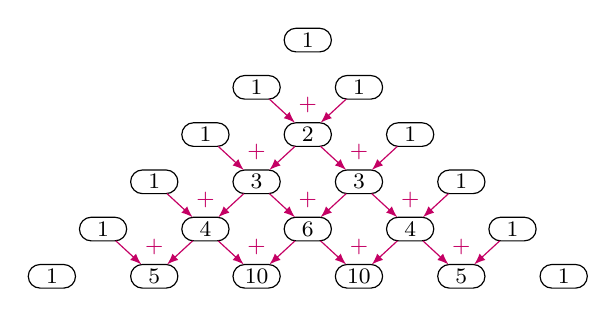
\begin{tikzpicture}[x=13mm,y=6mm]
  % some colors
  \colorlet{links}{sthlmRed}
  % some styles
  \tikzset{
    box/.style={
      minimum height=3mm,
      inner sep=.5mm,
      outer sep=0mm,
      text width=5mm,
      text centered,
      font=\footnotesize,
      draw=#1,
      line width=.15mm,
      rounded corners=1.5mm,
    },
    link/.style={-latex,links,line width=.15mm},
    plus/.style={text=links,font=\footnotesize},
  }
  % Pascal's triangle
  % row #0 => value is 1

  \node[box] (p-0-0) at (0,0) {1};
  \foreach \row in {1,...,5} {
     % col #0 =&gt; value is 1
    \node[box] (p-\row-0) at (-\row/2,-\row) {1};
    \pgfmathsetmacro{\molson}{1};
    \foreach \col in {1,...,\row} {
      % iterative formula : val = precval * (row-col+1)/col
      % (+ 0.5 to bypass rounding errors)
      \pgfmathtruncatemacro{\molson}{\molson*((\row-\col+1)/\col)+0.5};
      \global\let\molson=\molson
      % position of each molson
      \coordinate (pos) at (-\row/2+\col,-\row);
        \node[box] (p-\row-\col) at (pos) {\molson};
      % for arrows and plus sign
      \ifnum \col<\row
        \node[plus,above=0mm of p-\row-\col]{+};
        \pgfmathtruncatemacro{\prow}{\row-1}
        \pgfmathtruncatemacro{\pcol}{\col-1}
        \draw[link] (p-\prow-\pcol) -- (p-\row-\col);
        \draw[link] (p-\prow-\col) -- (p-\row-\col);
      \fi
    }
  }
\end{tikzpicture}
\end{mysection}

\begin{mysection}{Pythagorean Theorem}
\begin{multicols}{2}
\begin{tabular}{@{}ll@{}}

\cRed{PyThm}	& \texttt{Pythagorean Theorem}	\\
	 				& $a^2+b^2=c^2$
\end{tabular}

\columnbreak

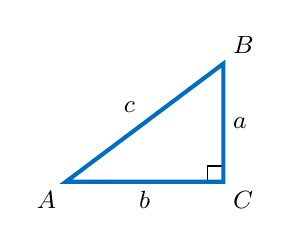
\begin{tikzpicture}[scale=0.5]
   \fill [fill=white] (0,0) -- (4,0) -- (4,3) -- (0,0);
   \draw [line width=0.5pt] (3.6,0) -- (3.6,0.4) -- (4,0.4);
   \draw [color=sthlmBlue,line width=1.5pt] (0,0) -- (4,0) -- (4,3) -- cycle;
   \node [below left] at (0,0) {\small $A$};
   \node [below right] at (4,0) {\small $C$};
   \node [above right] at (4,3) {\small $B$};
   \node [below] at (2,0) {\small $b$};
   \node [right] at (4,1.5) {\small $a$};
   \node [above left] at (2,1.5) {\small $c$};
  \end{tikzpicture}
\end{multicols}
\end{mysection}

\begin{mysection}{Function}

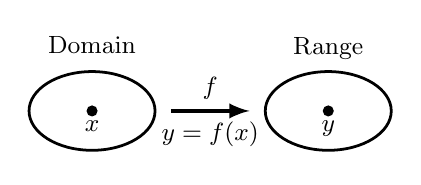
\begin{tikzpicture}[every node/.style={font=\small}]
 \draw [line width=1pt] (0,0) ellipse (0.8 and 0.5);
 \fill (0,0) circle (2pt);
 \node [below] at (0,0) {$x$};
 \node [above] at (0,0.6) {Domain};
 \draw [line width=1pt] (3,0) ellipse (0.8 and 0.5);
 \fill (3,0) circle (2pt);
 \node [below] at (3,0) {$y$};
 \node [above] at (3,0.53) {Range};
 \draw [-latex,line width=1.5pt] (1,0) -- (2,0) node[midway,above] {$f$}
  node[midway,below] {$y=f(x)$};
\end{tikzpicture}

\end{mysection}

\begin{mysection}{Function Vertical Line Test}

\begin{tabular}{@{}ll@{}l@{}}
\cRed{FVLT}		& \texttt{Function Vertical Line Test} \\
						&
\end{tabular}

\begin{multicols}{2}

  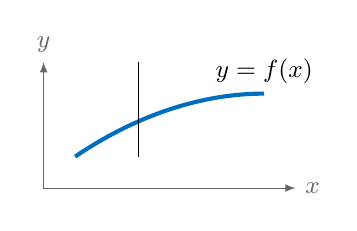
\begin{tikzpicture}[scale=0.8,every node/.style={font=\small}]
   \draw[latex-latex,black!60,line width=0.3pt] (0,2) node[above] {$y$} |- (4,0) node[right] {$x$};
   \draw [sthlmBlue,line width=1.5pt] (0.5,0.5) parabola[bend at end] (3.5,1.5);
   \node[above] at (3.5,1.5) {$y=f(x)$};
   \draw (1.5,0.5) -- (1.5,2);
  \end{tikzpicture}
\quad $f$ is a function
\columnbreak

  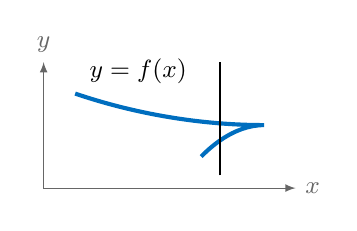
\begin{tikzpicture}[scale=0.8, every node/.style={font=\small}]
   \draw[latex-latex,black!60,line width=0.3pt] (0,2) node[above] {$y$} |- (4,0) node[right] {$x$};
   \draw [sthlmBlue,line width=1.5pt] (0.5,1.5) parabola bend  (3.5,1) (2.5,0.5);
   \node[above] at (1.5,1.5) {$y=f(x)$};
   \draw (2.8,0.2) -- (2.8,2);
  \end{tikzpicture}
\quad $f$ is not a function
\end{multicols}
\end{mysection}

 \begin{mysection}{Horizontal Line Test}
 \begin{tabular}{@{}ll@{}l@{}}
 \cRed{FHLT}		& \texttt{Function Horizontal Line Test}
 \end{tabular}

 \begin{multicols}{2}
  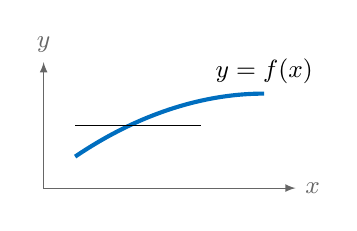
\begin{tikzpicture}[scale=0.8,every node/.style={font=\small}]
   \draw[latex-latex,black!60,line width=0.3pt] (0,2) node[above] {$y$} |- (4,0) node[right] {$x$};
   \draw [sthlmBlue,line width=1.5pt] (0.5,0.5) parabola[bend at end] (3.5,1.5);
   \node[above] at (3.5,1.5) {$y=f(x)$};
   \draw (0.5,1) -- (2.5,1);
  \end{tikzpicture}
  \quad $f$ is one-to-one
  \columnbreak

  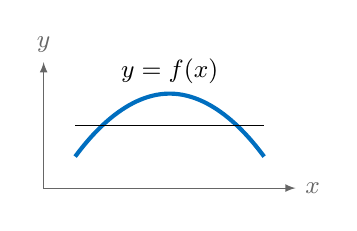
\begin{tikzpicture}[scale=0.8,every node/.style={font=\small}]
   \draw[latex-latex,black!60,line width=0.3pt] (0,2) node[above] {$y$} |- (4,0) node[right] {$x$};
   \draw [sthlmBlue,line width=1.5pt] (0.5,0.5) parabola bend  (2,1.5) (3.5,0.5);
   \node[above] at (2,1.5) {$y=f(x)$};
   \draw (0.5,1) -- (3.5,1);
  \end{tikzpicture}
  \quad $f$ is not one-to-one

 \end{multicols}
 \end{mysection}


\begin{mysection}{Linear Functions}
  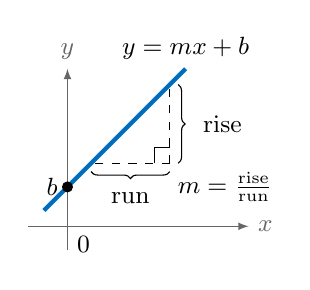
\begin{tikzpicture}[every node/.style={font=\small}]
   \draw [black!60,line width=0.3pt,-latex] (-0.5,0) -- (2.3,0) node [right] {$x$};
   \draw [black!60,line width=0.3pt,-latex] (0,-0.3) -- (0,2) node [above] {$y$};
   \node [below right] at (0,0) {$0$};
   \draw [dashed] (1.3,0.8) -- (0.3,0.8);
   \draw [dashed] (1.3,0.8) -- (1.3,1.8);
   \draw [color=sthlmBlue,line width=1.5pt] (-0.3,0.2) -- (1.5,2);
   \node [above] at (1.5,2) {$y=mx+b$};
   \fill (0,0.5) circle (2pt);
   \node [left] at (0,0.5) {$b$};
   \draw (1.1,0.8) -- (1.1,1) -- (1.3,1);
   \draw [decorate,decoration={brace,raise=3pt,mirror}]
	(0.3,0.8) -- (1.3,0.8);
   \draw [decorate,decoration={brace,raise=3pt,mirror}]
	(1.3,0.8) -- (1.3,1.8);
   \node [below] at (0.8,0.55) {run};
   \node [right] at (1.6,1.3) {rise};
   \node at (2,0.5) {$m = \frac{\text{rise}}{\text{run}}$};
  \end{tikzpicture}



\begin{tabular}{@{}ll@{}}
\cRed{DBP}			& \texttt{Distance betweent $P_1=(x_1, y_1)$} \\
						& \texttt{\& $P_2=(x_2, y_2)$} \\
						& \qquad $d \left(P_1, P_2 \right)=\sqrt{(x_2-x_1)^2+(y_2-y_1)^2}$\\
						& \\
\cRed{MBP}			& \texttt{Midpoint between $P_1=(x_1, y_1)$} \\
						& \texttt{\& $P_2=(x_2, y_2)$} \\
						& \qquad $\text{Midpoint of }P_1P_2= \left(\frac{x_1+x_2}{2}, \frac{y_1+y_2}{3} \right)$\\
						& \\
\cRed{Line Slope}	& \texttt{Line Slope through $P_1=(x_1, y_1)$} \\
						& \texttt{\& $P_2=(x_2, y_2)$ } \\
						& \qquad $m=\frac{y_2-y_1}{x_2-x_1}$\\
						& \\
\cRed{PSE}			& \texttt{Point slope equation though $P(x_1, y_2)$} \\
						& \qquad $y-y_1=m(x-x_1)$\\
						& \\
\cRed{SIE}			& \texttt{Slope-intercept equation } \\
						& \qquad $y=mx+b$ \\
						& \\
\cRed{PrSPL}		& \texttt{Product of slopes - Perpendicual Lines } \\
						& \qquad $m_1 m_2 =-1$
\end{tabular}

  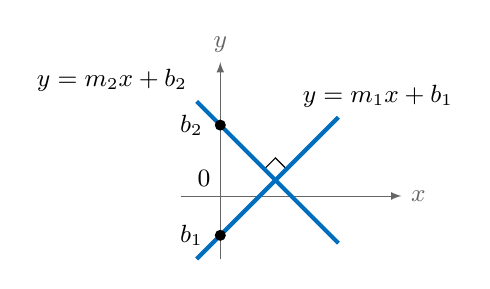
\begin{tikzpicture}[every node/.style={font=\small}]
   \draw [black!60,line width=0.3pt,-latex] (-0.5,0) -- (2.3,0) node [right] {$x$};
   \draw [black!60,line width=0.3pt,-latex] (0,-0.8) -- (0,1.7) node [above] {$y$};
   \node [above left] at (0,0) {$0$};
   \draw [rotate around={45:(0.7,0.2)}] (0.9,0.2) -- (0.9,0.4) -- (0.7,0.4);
   \draw [color=sthlmBlue,line width=1.5pt] (-0.3,-0.8) -- (1.5,1.0);
   \draw [color=sthlmBlue,line width=1.5pt] (-0.3,1.2) -- (1.5,-0.6);
   \node [above] at (2,1.0) {$y=m_{1}x+b_1$};
   \fill (0,-0.5) circle (2pt);
   \node [left] at (-0.1,-0.5) {$b_1$};
   \node [above left] at (-0.3,1.2) {$y=m_{2}x+b_2$};
   \fill (0,0.9) circle (2pt);
   \node [left] at (-0.1,0.9) {$b_2$};
  \end{tikzpicture}
 \end{mysection}

\begin{mysection}{Quadratic Functions}
 If $ax^2+bx+c=0$, where $a \ne 0$, then \\

 \[
 x= \dfrac{-b\pm \sqrt{b^2-4ac}}{2a}
 \]

 \begin{enumerate}
 	\item $b^2-4ac>0$ Two distinct real solutions
 	\item $b^2-4ac=0$ Two repeated real solutions
 	\item $b^2-4ac<0$ Two distinct complex solutions
 \end{enumerate}
 \end{mysection}


\begin{mysection}{Greek Alphabet}

\begin{tabular}{lllllllll}
\multicolumn{2}{l}{\textbf{Letters}} & \textbf{Name} & \multicolumn{2}{l}{\textbf{Letters}} &\textbf{Name} \\[4pt]
A & $\alpha$ & \texttt{alpha}			& N & $\nu$ & \texttt{nu} \\
B & $\beta$ & \texttt{beta} 			& $\Xi$ & $\xi$ & \texttt{xi} \\
$\Gamma$ & $\gamma$ & \texttt{gamma} 	& O & $o$ & \texttt{omicron} \\
$\Delta$ & $\delta$ & \texttt{delta} 	& $\Pi$ & $\pi$ & \texttt{pi}\\
E & $\epsilon$ & \texttt{epsilon} 		& P & $\rho$ & \texttt{rho}\\
Z & $\zeta$ & \texttt{zeta} 			& $\Sigma$ & $\sigma$ & \texttt{sigma}\\
H & $\eta$ & \texttt{eta} 				& T & $\tau$ & \texttt{tau}\\
$\Theta$ & $\theta$ & \texttt{theta} 	& $\Upsilon$ & $\upsilon$ & \texttt{upsilon}\\
I & $\iota$ & \texttt{iota} 			& $\Phi$ & $\phi$ & \texttt{phi}\\
K & $\kappa$ & \texttt{kappa} 			& X & $\chi$ & \texttt{chi}\\
$\Lambda$ & $\lambda$ & \texttt{lambda}	& $\Psi$ & $\psi$ & \texttt{psi}\\
M & $\mu$ & \texttt{mu} 				& $\Omega$ & $\omega$ & \texttt{omega}
\end{tabular}
\end{mysection}

\begin{mysection}{Angles: Components}

 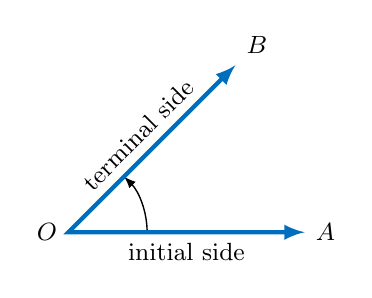
\begin{tikzpicture}
  \draw [line width=0.5pt,-latex] (1,0) arc (0:45:1);
  \draw [color=sthlmBlue,line width=1.5pt,latex-latex] (3,0) node[black,right] {\small $A$} -- (0,0)
  node[black,left] {\small $O$} node[black,midway,below] {\small initial side} --
  (2.1213,2.1213) node[black,above right] {\small $B$} node[black,midway,sloped,above]
  {\small terminal side};
 \end{tikzpicture}
\end{mysection}

\begin{mysection}{Angle Direction \& Magnitude}

 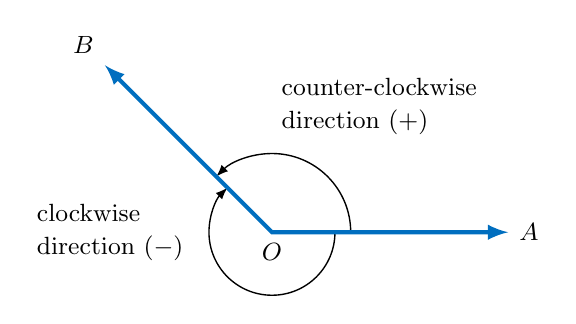
\begin{tikzpicture}
  \draw [line width=0.5pt,-latex] (1,0) arc (0:135:1);
  \node[right,align=left] at (0,1.6) {\small counter-clockwise\\\small direction ($+$)};
  \draw [line width=0.5pt,-latex] (0.8,0) arc (360:135:0.8);
  \node[left,align=left] at (-1,0) {\small clockwise\\\small direction ($-$)};
  \draw [color=sthlmBlue,line width=1.5pt,latex-latex] (3,0) node[black,right] {\small $A$} --
  (0,0) node[black,below] {\small $O$} -- (-2.1213,2.1213) node[black,above left] {\small $B$};
 \end{tikzpicture}
\end{mysection}

\begin{mysection}{Radians}

 \begin{multicols}{2}
 \begin{tabular}{@{}ll@{}}

 \cRed{Rad}	& \texttt{Radian}	\\
 	 				& $1 \text{ radian}= \frac{180}{\pi} \approx 57.3 \degree$

 \end{tabular}

 \columnbreak

 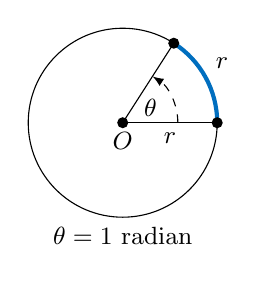
\begin{tikzpicture}[every node/.style={font=\small}]
  \draw (0,0) circle (1.2);
  \fill (0,0) circle (2pt);
  \node [below] at (0,0) {$O$};
  \draw (0,0) -- (0:1.2) node[below,midway] {$r$};
  \draw (0,0) -- (57.3:1.2);
  \draw [color=sthlmBlue,line width=1.5pt] (0:1.2) arc (0:57.3:1.2);
  \fill (0:1.2) circle (2pt);
  \fill (57.3:1.2) circle (2pt);
  \node [above right] at (28:1.2) {$r$};
  \node at (28:0.4) {$\theta$};
  \draw [dashed,-latex] (0:0.7) arc (0:57.3:0.7);
  \node [below] at (270:1.2) {$\theta = 1$ radian};
 \end{tikzpicture}
 \end{multicols}
\end{mysection}


\begin{mysection}{Arc Length and Sector Area}

 \begin{multicols}{2}
 \begin{tabular}{@{}ll@{}}

 \cRed{AL}	& \texttt{Arc Length}	\\
 	 				& $s= r \theta $ \\
					& \\
 \cRed{ASect}	& \texttt{Area of a Sector}	\\
 	 				& $A = \frac{1}{2}r^2 \theta $
 \end{tabular}

 \columnbreak

   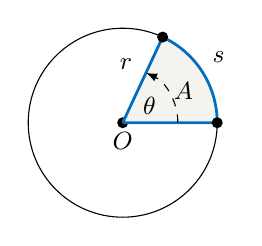
\begin{tikzpicture}[every node/.style={font=\small}]
    \draw (0,0) circle (1.2);
    \fill (0,0) circle (2pt);
    \node [below] at (0,0) {$O$};
    \draw (0,0) -- (65:1.2);
  \filldraw [color=sthlmBlue,fill=sthlmGrey,line width=1pt] (0,0) -- (65:1.2)
   node[black,midway,above left] {$r$} arc (65:0:1.2) -- (0,0);
    \fill (0:1.2) circle (2pt);
    \fill (65:1.2) circle (2pt);
    \node [above right] at (32:1.2) {$s$};
	\node [below left] at (32:1.2) {$A$};
    \node at (32:0.4) {$\theta$};
    \draw [dashed,-latex] (0:0.7) arc (0:65:0.7);
   \end{tikzpicture}
 \end{multicols}
\end{mysection}


\begin{mysection}{Classification of Angles}

\begin{multicols}{2}
\begin{tabular}{@{}ll@{}}

\cRed{AA}	& \texttt{Acute Angle}
\end{tabular}

\columnbreak

 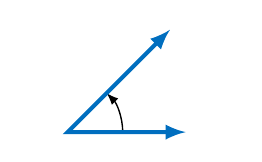
\begin{tikzpicture}
  \draw [line width=0.5pt,-latex] (0.7,0) arc (0:45:0.7);
  \draw [color=sthlmBlue,line width=1.5pt,latex-latex] (1.5,0) -- (0,0) -- (1.3,1.3);
  \draw [white] (1.6,0) -- (2.1,0);
  \draw [white] (-0.1,0) -- (-0.5,0);
 \end{tikzpicture}

\end{multicols}

\vspace{0.75cm}

\begin{multicols}{2}
\begin{tabular}{@{}ll@{}}

\cRed{RA}	& \texttt{Right Angle}
\end{tabular}

\columnbreak

 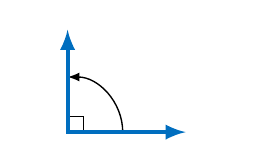
\begin{tikzpicture}
  \draw [line width=0.5pt,-latex] (0.7,0) arc (0:90:0.7);
  \draw [line width=0.5pt] (0.2,0) -- (0.2,0.2) -- (0,0.2);
  \draw [color=sthlmBlue,line width=1.5pt,latex-latex] (1.5,0) -- (0,0) -- (0,1.3);
  \draw [white] (1.6,0) -- (2.1,0);
  \draw [white] (-0.1,0) -- (-0.5,0);
 \end{tikzpicture}

\end{multicols}

\vspace{0.75cm}

\begin{multicols}{2}
\begin{tabular}{@{}ll@{}}

\cRed{OA}	& \texttt{Obtuse Angle}
\end{tabular}

\columnbreak

 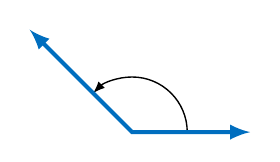
\begin{tikzpicture}
  \draw [line width=0.5pt,-latex] (0.7,0) arc (0:135:0.7);
  \draw [color=sthlmBlue,line width=1.5pt,latex-latex] (1.5,0) -- (0,0) -- (-1.3,1.3);
 \end{tikzpicture}

\end{multicols}

\vspace{0.75cm}
\begin{multicols}{2}
\begin{tabular}{@{}ll@{}}

\cRed{SA}	& \texttt{Straight Angle}
\end{tabular}

\columnbreak

 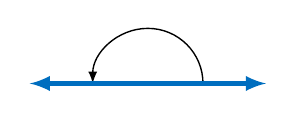
\begin{tikzpicture}
  \draw [line width=0.5pt,-latex] (0.7,0) arc (0:180:0.7);
  \draw [color=sthlmBlue,line width=1.5pt,latex-latex] (-1.5,0) -- (0,0) -- (1.5,0);
 \end{tikzpicture}

\end{multicols}
\vspace{0.75cm}
\end{mysection}

\begin{mysection}{Angle Pairings}

\begin{multicols}{2}
\begin{tabular}{@{}ll@{}}

\cRed{ComA}	& \texttt{Complimentary Angles}
\end{tabular}

\columnbreak

 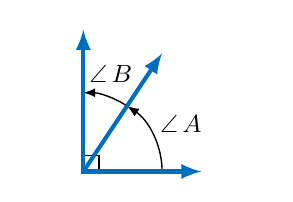
\begin{tikzpicture}
  \draw [line width=0.5pt,latex-] (0,1) arc (90:56.3:1);
  \draw [line width=0.5pt,-latex] (1,0) arc (0:56.3:1);
  \draw [line width=0.5pt] (0.2,0) -- (0.2,0.2) -- (0,0.2);
  \draw [color=sthlmBlue,line width=1.5pt,latex-latex] (1.5,0) -- (0,0) -- (0,1.8);
  \draw [color=sthlmBlue,line width=1.5pt,-latex] (0,0) -- (1,1.5);
  \draw [white] (1.6,0) -- (2.3,0);
  \draw [white] (-0.1,0) -- (-0.7,0);
  \node [right] at (0.85,0.6) {\small $\angle\,A$};
  \node [above] at (0.35,1) {\small $\angle\,B$};
 \end{tikzpicture}

\end{multicols}

\vspace{0.75cm}

\begin{multicols}{2}
\begin{tabular}{@{}ll@{}}

\cRed{SA}	& \texttt{Supplementary Angles}
\end{tabular}

\columnbreak

 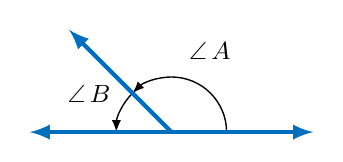
\begin{tikzpicture}
  \draw [line width=0.5pt,-latex] (0.7,0) arc (0:135:0.7);
  \draw [line width=0.5pt,latex-] (-0.7,0) arc (180:135:0.7);
  \draw [color=sthlmBlue,line width=1.5pt,latex-latex] (-1.8,0) -- (1.8,0);
  \draw [color=sthlmBlue,line width=1.5pt,-latex] (0,0) -- (-1.3,1.3);
  \node [above right] at (0.1,0.8) {\small $\angle\,A$};
  \node [above left] at (-0.65,0.25) {\small $\angle\,B$};
 \end{tikzpicture}

\end{multicols}

\vspace{0.75cm}

\begin{multicols}{2}
\begin{tabular}{@{}ll@{}}

\cRed{ConA}	& \texttt{Conjugate Angles}
\end{tabular}

\columnbreak

 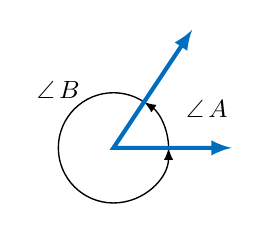
\begin{tikzpicture}
  \draw [line width=0.5pt,latex-] (0.7,0) arc (360:56.3:0.7);
  \draw [line width=0.5pt,-latex] (0.7,0) arc (0:56.3:0.7);
  \draw [color=sthlmBlue,line width=1.5pt,latex-latex] (1.5,0) -- (0,0) -- (1,1.5);
  \node [right] at (0.8,0.5) {\small $\angle\,A$};
  \node [above] at (-0.7,0.5) {\small $\angle\,B$};
 \end{tikzpicture}

\end{multicols}
\end{mysection}

\begin{mysection}{Trigonometric Function Definitions}
\begin{multicols}{2}

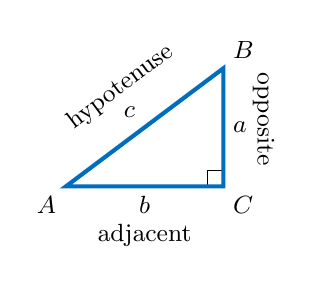
\begin{tikzpicture}[scale=0.5]
   \fill [fill=white] (0,0) -- (4,0) -- (4,3) -- (0,0);
   \draw [line width=0.5pt] (3.6,0) -- (3.6,0.4) -- (4,0.4);
   \draw [color=sthlmBlue,line width=1.5pt] (0,0) -- (4,0) -- (4,3) -- cycle;
   \node [below left] at (0,0) {\small $A$};
   \node [below right] at (4,0) {\small $C$};
   \node [above right] at (4,3) {\small $B$};
   \node [below] at (2,0) {\small $b$};
   \node [below] at (2,-0.7) {\small adjacent};
   \node [right] at (4,1.5) {\small $a$};
   \node [rotate=-90,above] at (4.5,1.7) {\small opposite};
   \node [above left] at (2,1.5) {\small $c$};
   \node [rotate=36.87,above] at (1.7,2.1) {\small hypotenuse};
  \end{tikzpicture}

\columnbreak

\begin{tabular}{l l }
$\sin A = \frac{\text{opp}}{\text{hyp}}$ & $\csc A = \frac{\text{hyp}}{\text{opp}}$ \\
& \\
$\cos A = \frac{\text{adj}}{\text{hyp}}$ & $\sec A = \frac{\text{hyp}}{\text{adj}}$ \\
& \\
$\tan A = \frac{\text{opp}}{\text{adj}}$ & $\cot A = \frac{\text{adj}}{\text{hyp}}$
\end{tabular}
\end{multicols}
\end{mysection}

\begin{mysection}{Unit Circle}
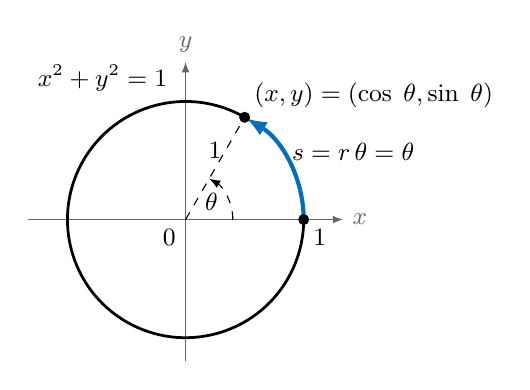
\begin{tikzpicture}[every node/.style={font=\small}]
 \draw[black!60,line width=0.3pt,-latex] (-2,0) -- (2,0) node[right] {$x$};
 \draw[black!60,line width=0.3pt,-latex] (0,-1.8) -- (0,2) node[above] {$y$};
 \draw [line width=1pt] (60:1.5) arc (60:360:1.5);
 \node [right] at (35:1.5) {$s=r\,\theta=\theta$};
 \draw [dashed] (0,0) -- (60:1.5) node[black,midway,above] {$1$};
 \draw [-latex,dashed] (0:0.6) arc (0:60:0.6);
 \draw [color=sthlmBlue,-latex,line width=1.5pt] (0:1.5) arc (0:59:1.5);
 \fill (0:1.5) circle (2pt);
 \fill (60:1.5) circle (2pt);
 \node at (35:0.4) {$\theta$};
 \node [below right] at (0:1.5) {$1$};
 \node [below left] at (0:0) {$0$};
 \node [above right] at (60:1.5) {$(x,y)=(\cos\;\theta,\sin\;\theta)$};
 \node [right] at (-2,1.8) {$x^2 + y^2 = 1$};
\end{tikzpicture}


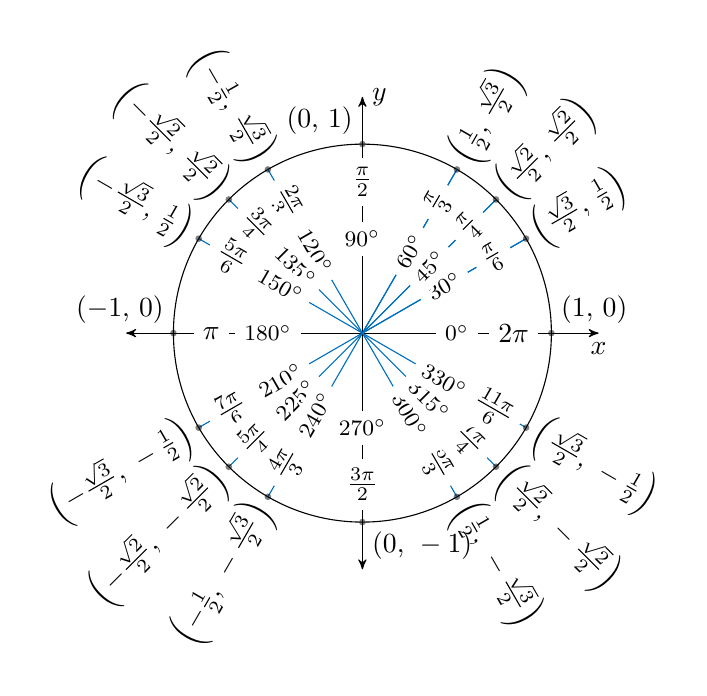
\begin{tikzpicture}[scale=2.4]
 \draw[<->] (-1.25,0) -- (1.25,0) node[anchor=north] {$x$};
 \draw [<->](0,-1.25) -- (0,1.25) node[anchor=west] {$y$};
 \draw (0,0) circle (1cm);
 \draw[sthlmBlue] (30:1cm) -- (0,0);
 \draw[sthlmBlue] (45:1cm) -- (0,0);
 \draw[sthlmBlue] (60:1cm) -- (0,0);

% 30 Degree Angle
\draw[sthlmBlue] (30:1cm) -- (0,0);
\node[anchor=west, rotate=30] (a1) at  ({cos(30)},{sin(30)}) {$\left(\frac{\sqrt{3}}{2} \text{, } \frac{1}{2} \right)$};
\node[rotate=30, fill=white] (a2) at ({cos(30)*.5}, {sin(30)*.5}) {\footnotesize{$30^{\circ}$}};
\node[rotate=30, fill=white] (a3) at ({cos(30)*.8}, {sin(30)*.8}) {\normalsize{$\frac{\pi}{6}$}};
\coordinate(a) at ({cos(30)},{sin(30)});
% 45 Degree Angle
\draw[sthlmBlue] (45:1cm) -- (0,0);
\node[anchor=west, rotate=45] (b1) at  ({cos(45)},{sin(45)}) {$\left(\frac{\sqrt{2}}{2} \text{, } \frac{\sqrt{2}}{2} \right)$};
\node[rotate=45, fill=white] (b2) at ({cos(45)*.5}, {sin(45)*.5}) {\footnotesize{$45^{\circ}$}};
\node[rotate=45, fill=white] (b3) at ({cos(45)*.8}, {sin(45)*.8}) {\normalsize{$\frac{\pi}{4}$}};
\coordinate(b) at ({cos(45)},{sin(45)});
% 60 Degree Angle
\draw[sthlmBlue] (60:1cm) -- (0,0);
\node[anchor=west, rotate=60] (c1) at  ({cos(60)},{sin(60)}) {$\left(\frac{1}{2} \text{, } \frac{\sqrt{3}}{2} \right)$};
\node[rotate=60, fill=white] (c2) at ({cos(60)*.5}, {sin(60)*.5}) {\footnotesize{$60^{\circ}$}};
\node[rotate=60, fill=white] (c3) at ({cos(60)*.8}, {sin(60)*.8}) {\normalsize{$\frac{\pi}{3}$}};
\coordinate(c) at ({cos(60)},{sin(60)});
% 90 Degree Angle
\node[anchor=west, above left] (d1) at  ({cos(90)},{sin(90)}) {$\left(0 \text{, } 1 \right)$};
\node[fill=white] (d2) at ({cos(90)*.5}, {sin(90)*.5}) {\footnotesize{$90^{\circ}$}};
\node[fill=white] (d3) at ({cos(90)*.8}, {sin(90)*.8}) {\normalsize{$\frac{\pi}{2}$}};
\coordinate(d) at ({cos(90)},{sin(90)});
% 120 Degree Angle
\draw[sthlmBlue] (120:1cm) -- (0,0);
\node[anchor=east, rotate=300] (e1) at  ({cos(120)},{sin(120)}) {$\left(-\frac{1}{2} \text{, } \frac{\sqrt{3}}{2} \right)$};
\node[rotate=300, fill=white] (e2) at ({cos(120)*.5}, {sin(120)*.5}) {\footnotesize{$120^{\circ}$}};
\node[rotate=300, fill=white] (e3) at ({cos(120)*.8}, {sin(120)*.8}) {\normalsize{$\frac{2\pi}{3}$}};
\coordinate(e) at ({cos(120)},{sin(120)});
% 135 Degree Angle
\draw[sthlmBlue] (135:1cm) -- (0,0);
\node[anchor=east, rotate=315] (f1) at  ({cos(135)},{sin(135)}) {$\left(-\frac{\sqrt{2}}{2} \text{, } \frac{\sqrt{2}}{2} \right)$};
\node[rotate=315, fill=white] (f2) at ({cos(135)*.5}, {sin(135)*.5}) {\footnotesize{$135^{\circ}$}};
\node[rotate=315, fill=white] (f3) at ({cos(135)*.8}, {sin(135)*.8}) {\normalsize{$\frac{3 \pi}{4}$}};
\coordinate(f) at ({cos(135)},{sin(135)});
% 150 Degree Angle
\draw[sthlmBlue] (150:1cm) -- (0,0);
\node[anchor=east, rotate=330] (g1) at  ({cos(150)},{sin(150)}) {$\left(-\frac{\sqrt{3}}{2} \text{, } \frac{1}{2} \right)$};
\node[rotate=330, fill=white] (g2) at ({cos(150)*.5}, {sin(150)*.5}) {\footnotesize{$150^{\circ}$}};
\node[rotate=330, fill=white] (g3) at ({cos(150)*.8}, {sin(150)*.8}) {\normalsize{$\frac{5 \pi}{6}$}};
\coordinate(g) at ({cos(150)},{sin(150)});
% 180 Degree Angle
\node[anchor=south, above left] (h1) at  ({cos(180)},{sin(180)}) {$\left(-1 \text{, } 0 \right)$};
\node[fill=white] (h2) at ({cos(180)*.5}, {sin(180)*.5}) {\footnotesize{$180^{\circ}$}};
\node[fill=white] (h3) at ({cos(180)*.8}, {sin(180)*.8}) {\normalsize{$\pi$}};
\coordinate(h) at ({cos(180)},{sin(180)});
% 210 Degree Angle
\draw[sthlmBlue] (210:1cm) -- (0,0);
\node[anchor=east, rotate=30] (i1) at  ({cos(210)},{sin(210)}) {$\left(-\frac{\sqrt{3}}{2} \text{, } -\frac{1}{2} \right)$};
\node[rotate=30, fill=white] (i2) at ({cos(210)*.5}, {sin(210)*.5}) {\footnotesize{$210^{\circ}$}};
\node[rotate=30, fill=white] (i3) at ({cos(210)*.8}, {sin(210)*.8}) {\normalsize{$\frac{7 \pi}{6}$}};
\coordinate(i) at ({cos(210)},{sin(210)});
% 225 Degree Angle
\draw[sthlmBlue] (225:1cm) -- (0,0);
\node[anchor=east, rotate=45] (j1) at  ({cos(225)},{sin(225)}) {$\left(-\frac{\sqrt{2}}{2} \text{, } -\frac{\sqrt{2}}{2} \right)$};
\node[rotate=45, fill=white] (j2) at ({cos(225)*.5}, {sin(225)*.5}) {\footnotesize{$225^{\circ}$}};
\node[rotate=45, fill=white] (j3) at ({cos(225)*.8}, {sin(225)*.8}) {\normalsize{$\frac{5 \pi}{4}$}};
\coordinate(j) at ({cos(225)},{sin(225)});
% 240 Degree Angle
\draw[sthlmBlue] (240:1cm) -- (0,0);
\node[anchor=east, rotate=60] (k1) at  ({cos(240)},{sin(240)}) {$\left(-\frac{1}{2} \text{, } -\frac{\sqrt{3}}{2} \right)$};
\node[rotate=60, fill=white] (k2) at ({cos(240)*.5}, {sin(240)*.5}) {\footnotesize{$240^{\circ}$}};
\node[rotate=60, fill=white] (k3) at ({cos(240)*.8}, {sin(240)*.8}) {\normalsize{$\frac{4\pi}{3}$}};
\coordinate(k) at ({cos(240)},{sin(240)});
% 270 Degree Angle
\node[anchor=east, below right] (l1) at  ({cos(270)},{sin(270)}) {$\left(0 \text{, } -1 \right)$};
\node[fill=white] (l2) at ({cos(270)*.5}, {sin(270)*.5}) {\footnotesize{$270^{\circ}$}};
\node[fill=white] (l3) at ({cos(270)*.8}, {sin(270)*.8}) {\normalsize{$\frac{3\pi}{2}$}};
\coordinate(l) at ({cos(270)},{sin(270)});
% 240 Degree Angle
\draw[sthlmBlue] (300:1cm) -- (0,0);
\node[anchor=west, rotate=300] (m1) at  ({cos(300)},{sin(300)}) {$\left(\frac{1}{2} \text{, } -\frac{\sqrt{3}}{2} \right)$};
\node[rotate=300, fill=white] (m2) at ({cos(300)*.5}, {sin(300)*.5}) {\footnotesize{$300^{\circ}$}};
\node[rotate=300, fill=white] (m3) at ({cos(300)*.8}, {sin(300)*.8}) {\normalsize{$\frac{5\pi}{3}$}};
\coordinate(m) at ({cos(300)},{sin(300)});
% 315 Degree Angle
\draw[sthlmBlue] (315:1cm) -- (0,0);
\node[anchor=west, rotate=315] (n1) at  ({cos(315)},{sin(315)}) {$\left(\frac{\sqrt{2}}{2} \text{, } -\frac{\sqrt{2}}{2} \right)$};
\node[rotate=315, fill=white] (n2) at ({cos(315)*.5}, {sin(315)*.5}) {\footnotesize{$315^{\circ}$}};
\node[rotate=315, fill=white] (n3) at ({cos(315)*.8}, {sin(315)*.8}) {\normalsize{$\frac{7 \pi}{4}$}};
\coordinate(n) at ({cos(315)},{sin(315)});
% 330 Degree Angle
\draw[sthlmBlue] (330:1cm) -- (0,0);
\node[anchor=west, rotate=330] (o1) at  ({cos(330)},{sin(330)}) {$\left(\frac{\sqrt{3}}{2} \text{, } -\frac{1}{2} \right)$};
\node[rotate=330, fill=white] (o2) at ({cos(330)*.5}, {sin(330)*.5}) {\footnotesize{$330^{\circ}$}};
\node[rotate=330, fill=white] (o3) at ({cos(330)*.8}, {sin(330)*.8}) {\normalsize{$\frac{11 \pi}{6}$}};
\coordinate(o) at ({cos(330)},{sin(330)});
% 360 Degree Angle
\node[anchor=south, above right] (p1) at  ({cos(0)},{sin(0)}) {$\left(1 \text{, } 0 \right)$};
\node[fill=white] (p2) at ({cos(0)*.5}, {sin(0)*.5}) {\footnotesize{$0^{\circ}$}};
\node[fill=white] (p3) at ({cos(0)*.8}, {sin(0)*.8}) {\normalsize{$2\pi$}};
\coordinate(p) at ({cos(0)},{sin(0)});
    \foreach \p in {a, b,c,d,e,f,g,h,i,j,k,l,m,n,o,p}
    \fill [opacity=.5] (\p) circle(.5pt);
\end{tikzpicture}
\end{mysection}

\begin{mysection}{Quadrants}
\begin{multicols}{2}

 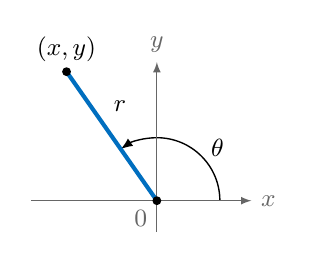
\begin{tikzpicture}[scale=0.8]
  \draw [line width=0.5pt,-latex] (1,0) arc (0:125:1);
  \draw [black!60,line width=0.3pt,-latex] (-2,0) -- (1.5,0) node [right] {\small $x$};
  \draw [black!60,line width=0.3pt,-latex] (0,-0.5) -- (0,2.2) node [above] {\small $y$};
  \node [black!60,below left] at (0,0) {\small $0$};
  \node [right] at (50:1.1) {\small $\theta$};
  \draw [color=sthlmBlue,line width=1.5pt] (0,0) -- (125:2.5) node[black,above right,pos=0.6] {\small $r$};
  \fill (0,0) circle (2pt);
  \fill (125:2.5) circle (2pt) node[above] {\small $(x,y)$};
 \end{tikzpicture}

\columnbreak

 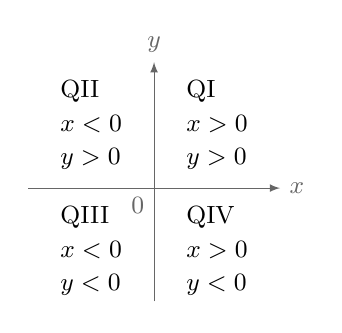
\begin{tikzpicture}[scale=0.8]
  \draw [black!60,line width=0.3pt,-latex] (-2,0) -- (2,0) node [right] {\small $x$};
  \draw [black!60,line width=0.3pt,-latex] (0,-1.8) -- (0,2) node [above] {\small $y$};
  \node [black!60,below left] at (0,0) {\small $0$};
  \node [align=left] at (1,1) {\small QI\\\small $x>0$\\\small $y>0$};
  \node [align=left] at (-1,1) {\small QII\\\small $x<0$\\\small $y>0$};
  \node [align=left] at (-1,-1) {\small QIII\\\small $x<0$\\\small $y<0$};
  \node [align=left] at (1,-1) {\small QIV\\\small $x>0$\\\small $y<0$};
 \end{tikzpicture}

\end{multicols}

  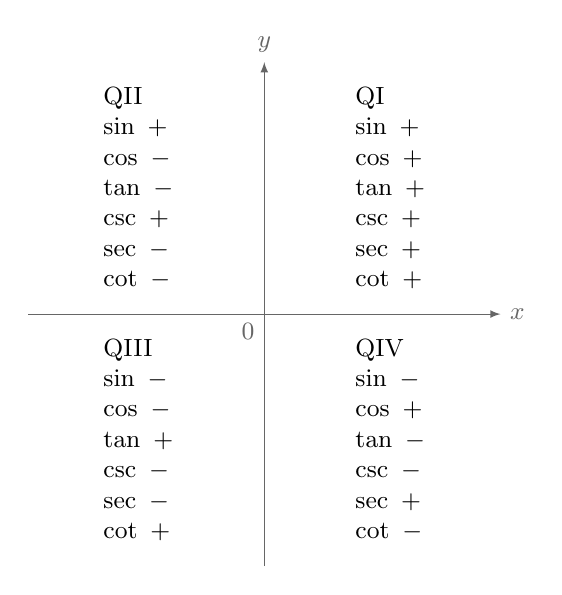
\begin{tikzpicture}[every node/.style={font=\small}]
  \draw [black!60,line width=0.3pt,-latex] (-3,0) -- (3,0) node [right] {$x$};
  \draw [black!60,line width=0.3pt,-latex] (0,-3.2) -- (0,3.2) node [above] {$y$};
  \node [black!60,below left] at (0,0) {$0$};
  \node [align=left] at (1.6,1.6)
   {QI\\$\sin~+$\\$\cos~+$\\$\tan~+$\\$\csc~+$\\$\sec~+$\\$\cot~+$};
  \node [align=left] at (-1.6,1.6)
   {QII\\$\sin~+$\\$\cos~-$\\$\tan~-$\\$\csc~+$\\$\sec~-$\\$\cot~-$};
  \node [align=left] at (-1.6,-1.6)
   {QIII\\$\sin~-$\\$\cos~-$\\$\tan~+$\\$\csc~-$\\$\sec~-$\\$\cot~+$};
  \node [align=left] at (1.6,-1.6)
   {QIV\\$\sin~-$\\$\cos~+$\\$\tan~-$\\$\csc~-$\\$\sec~+$\\$\cot~-$};
  \end{tikzpicture}

\end{mysection}

\begin{mysection}{Trigonometric Identities}
\begin{tabular}{@{}ll@{}}
\cRed{EOId}	& \texttt{Trigonometric Even/Odd Identities}	\\
&
\begin{tabular}{l l l }
$\sin -\theta = - \sin \theta $ & $\cos -\theta = \cos \theta $\\
& & \\
$\csc -\theta = - \csc \theta $ & $\sec -\theta = \sec \theta $ \\
& & \\
$\tan -\theta = - \tan \theta$ & $\cot -\theta = - \tan \theta$
\end{tabular} \\

& \\

\cRed{RId}	& \texttt{Trigonometric Reciprocal Identities}	\\
&
\begin{tabular}{l l l }
$\sin \theta = \frac{1}{\csc \theta}$ & $\cos \theta = \frac{1}{\sec \theta}$ & $\cot \theta = \frac{1}{\tan \theta}$ \\
& & \\
$\csc \theta = \frac{1}{\sin \theta}$ & $\sec \theta = \frac{1}{\cos \theta}$ & $\tan \theta = \frac{1}{\cot \theta}$
\end{tabular} \\

& \\

\cRed{PyId}	& \texttt{Trigonometric Pythagorean Identities}	\\

&
\begin{tabular}{l l }
$\sin^2 \theta + \cos^2 \theta = 1$ & \\
&  \\
 $\sec^2 \theta = \tan^2 \theta +1$ & $\csc^2 \theta = 1 + \cot^2 \theta$
\end{tabular}\\

& \\

\cRed{TanId}	& \texttt{Tangent Identity}	\\

& $\tan \theta = \frac{\sin \theta}{\cos \theta}$ \\

& \\

\cRed{CotId}	& \texttt{Cotangent Identity}	\\

& $\cot \theta = \frac{\cos \theta}{\sin \theta}$ \\

& \\

\cRed{SinDAId}	& \texttt{Sine Double Angle Identity}	\\

& $\sin 2\theta = 2 \sin \theta \cos \theta$ \\

& \\

\cRed{CosDAId}	& \texttt{Cosine Double Angle Identity}	\\

& $\cos 2\theta = \cos^2 \theta - \sin^2 \theta$ \\
& $\phantom{\cos 2\theta} =  1-2 \sin^2 \theta$\\
& $\phantom{\cos 2\theta} =  2 \cos^2 \theta-1$\\
& \\

\cRed{TanDAId}	& \texttt{Tangent Double Angle Identity}	\\

& $\tan 2\theta = \frac{2 \tan \theta}{1-\tan^2 \theta}$ \\

& \\

\cRed{SinSAId}	& \texttt{Sine Sum of Angles Identity}	\\

& $\sin (\theta + \phi)= \sin \theta \cos \phi + \cos \theta \sin \phi$ \\

& \\

\cRed{SinDiffAId}	& \texttt{Sine Difference of Angles Identity}	\\

& $\sin (\theta - \phi)= \sin \theta \cos \phi - \cos \theta \sin \phi$ \\

& \\

\cRed{CosSAId}	& \texttt{Cosine Sum of Angles Identity}	\\

& $\cos (\theta + \phi)= \cos \theta \cos \phi - \sin \theta \sin \phi$ \\

& \\

\cRed{CosDAId}	& \texttt{Cosine Difference of Angles Identity}	\\

& $\cos (\theta - \phi)= \cos \theta \cos \phi + \sin \theta \sin \phi$ \\

& \\

\cRed{TanSAId}	& \texttt{Tangent Sum of Angles Identity}	\\

& $\tan (\theta + \phi)= \dfrac{\tan \theta + \tan \phi}{1- \tan \theta \tan \phi}$ \\

& \\

\cRed{TanDiffAId}	& \texttt{Tangent Difference of Angles Identity}	\\

& $\tan (\theta - \phi)= \dfrac{\tan \theta - \tan \phi}{1+ \tan \theta \tan \phi}$ \\

&

\end{tabular}

\end{mysection}

\begin{mysection}{Cosine Law}

\begin{tabular}{@{}ll@{}}
\cRed{CL}	& \texttt{Cosine Law}	\\
&
\begin{tabular}{l l }
$a^2=b^2+c^2-2bc \cos A$ & $\cos A = \dfrac{b^2+c^2-a^2}{2bc}$ \\
& \\
$b^2= a^2+c^2 - 2ac \cos B$ & $\cos B = \dfrac{a^2+c^2-b^2}{2ac}$ \\
& \\
$c^2= a^2+b^2 - 2ab \cos C$ & $\cos C = \dfrac{a^2+b^2-c^2}{2ab}$ \\
\end{tabular}
\end{tabular}

\begin{multicols}{2}
  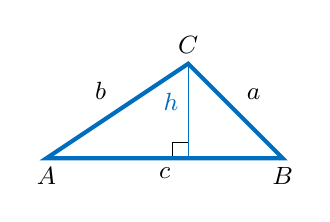
\begin{tikzpicture}[scale=1,every node/.style={font=\small}]
   \fill [white] (0,0) -- (1.8,1.2) -- (3,0) -- cycle;
   \draw [color=sthlmBlue] (1.8,1.2) -- (1.8,0) node[pos=0.4,left] {$h$};
   \draw (1.6,0) -- (1.6,0.2) -- (1.8,0.2);
   \draw [color=sthlmBlue,line width=1.5pt] (0,0) -- (1.8,1.2) node[black,midway,above left] {$b$} --
    (3,0) node[black,midway,above right] {$a$} -- cycle;
   \node [below] at (0,0) {$A$};
   \node [above] at (1.8,1.2) {$C$};
   \node [below] at (3,0) {$B$};
   \node [below] at (1.5,0) {$c$};
  \end{tikzpicture}

  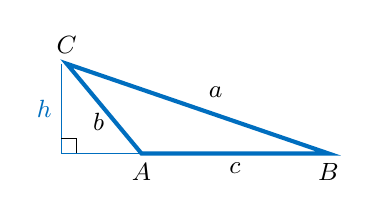
\begin{tikzpicture}[scale=0.95,every node/.style={font=\small}]
   \fill [white] (0,0) -- (-1,1.2) -- (2.5,0) -- cycle;
   \draw [color=sthlmBlue] (-1.07,1.2) -- (-1.07,0) node[midway,left] {$h$} -- (0,0);
   \draw (-0.87,0) -- (-0.87,0.2) -- (-1.07,0.2);
   \draw [color=sthlmBlue,line width=1.5pt] (0,0) -- (-1,1.2) node[black,pos=0.35,left] {$b$} --
    (2.5,0) node[black,midway,above right] {$a$} -- cycle;
   \node [below] at (0,0) {$A$};
   \node [above] at (-1,1.2) {$C$};
   \node [below] at (2.5,0) {$B$};
   \node [below] at (1.25,0) {$c$};
  \end{tikzpicture}
\end{multicols}
\end{mysection}

\begin{mysection}{Sine Law}
\begin{tabular}{@{}ll@{}}
\cRed{SL}	& \texttt{Sine Law}	\\
&
$\dfrac{\sin A}{a}=\dfrac{\sin B}{ b}=\dfrac{\sin C }{c}$
\end{tabular}

\begin{multicols}{2}
  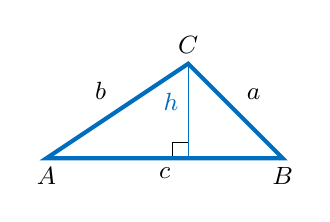
\begin{tikzpicture}[scale=1,every node/.style={font=\small}]
   \fill [white] (0,0) -- (1.8,1.2) -- (3,0) -- cycle;
   \draw [color=sthlmBlue] (1.8,1.2) -- (1.8,0) node[pos=0.4,left] {$h$};
   \draw (1.6,0) -- (1.6,0.2) -- (1.8,0.2);
   \draw [color=sthlmBlue,line width=1.5pt] (0,0) -- (1.8,1.2) node[black,midway,above left] {$b$} --
    (3,0) node[black,midway,above right] {$a$} -- cycle;
   \node [below] at (0,0) {$A$};
   \node [above] at (1.8,1.2) {$C$};
   \node [below] at (3,0) {$B$};
   \node [below] at (1.5,0) {$c$};
  \end{tikzpicture}

  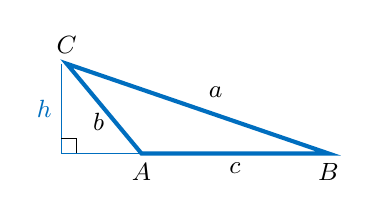
\begin{tikzpicture}[scale=0.95,every node/.style={font=\small}]
   \fill [white] (0,0) -- (-1,1.2) -- (2.5,0) -- cycle;
   \draw [color=sthlmBlue] (-1.07,1.2) -- (-1.07,0) node[midway,left] {$h$} -- (0,0);
   \draw (-0.87,0) -- (-0.87,0.2) -- (-1.07,0.2);
   \draw [color=sthlmBlue,line width=1.5pt] (0,0) -- (-1,1.2) node[black,pos=0.35,left] {$b$} --
    (2.5,0) node[black,midway,above right] {$a$} -- cycle;
   \node [below] at (0,0) {$A$};
   \node [above] at (-1,1.2) {$C$};
   \node [below] at (2.5,0) {$B$};
   \node [below] at (1.25,0) {$c$};
  \end{tikzpicture}
\end{multicols}
\end{mysection}

\begin{mysection}{Summary of the Ambiguous Case}

%\section{$90\degree \le A < 180\degree$}
%\vspace{0.5cm}

\cRed{$90\degree \le A < 180\degree$, $a > b$ :  One solution}

\begin{center}
    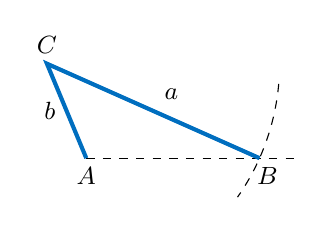
\begin{tikzpicture}[scale=1,every node/.style={font=\small}]
     \draw [dashed] (0,0) -- (2.7,0);
     \draw [dashed] ([shift={(-0.5,1.2)}] -5:2.955) arc (-5:-35:2.955);
     \draw [color=sthlmBlue,line width=1.5pt] (0,0) -- (-0.5,1.2) node[black,midway,left] {$b$} --
      (2.2,0) node[black,midway,above right] {$a$};
     \node [below] at (0,0) {$A$};
     \node [above] at (-0.5,1.2) {$C$};
     \node [below] at (2.3,0) {$B$};
    \end{tikzpicture}
\end{center}

\cRed{$90\degree \le A < 180\degree$, $a \le b$ : No solution}

\begin{center}
  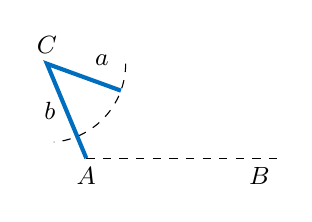
\begin{tikzpicture}[scale=1,every node/.style={font=\small}]
   \draw [dashed] (0,0) -- (2.5,0);
   \draw [dashed] ([shift={(-0.5,1.2)}] 0:1) arc (0:-85:1);
   \draw [color=sthlmBlue,line width=1.5pt] (0,0) -- (-0.5,1.2) node[black,midway,left] {$b$} --
    ++(-20:1) node[black,midway,above right] {$a$};
   \node [below] at (0,0) {$A$};
   \node [above] at (-0.5,1.2) {$C$};
   \node [below] at (2.2,0) {$B$};
  \end{tikzpicture}
\end{center}

%\section{$0\degree < A < 90\degree$}
%\vspace{0.5cm}

 \cRed{$0\degree < A < 90\degree$, $a < b\;\sin\;A$ :  No solution}
 \begin{center}
  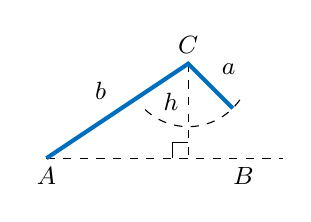
\begin{tikzpicture}[scale=1,every node/.style={font=\small}]
   \draw [dashed] (0,0) -- (3,0);
   \draw [dashed] (1.8,1.2) -- (1.8,0) node[pos=0.4,left] {$h$};
   \draw (1.6,0) -- (1.6,0.2) -- (1.8,0.2);
   \draw [dashed] ([shift={(1.8,1.2)}] -35:0.8) arc (-35:-135:0.8);
   \draw [color=sthlmBlue,line width=1.5pt] (0,0) -- (1.8,1.2) node[black,midway,above left] {$b$} --
    ++(-45:0.8) node[black,midway,above right] {$a$};
   \node [below] at (0,0) {$A$};
   \node [above] at (1.8,1.2) {$C$};
   \node [below] at (2.5,0) {$B$};
  \end{tikzpicture}
  \end{center}

  \cRed{$0\degree < A < 90\degree$, $a = b\;\sin\;A$ :  One solution}
  \begin{center}
  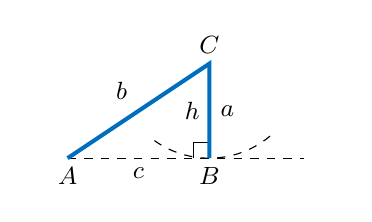
\begin{tikzpicture}[scale=1,every node/.style={font=\small}]
   \draw [white] (-0.5,0) -- (3.5,0);
   \draw [dashed] (0,0) -- (3,0);
   \draw [dashed] (1.8,1.2) -- (1.8,0) node[midway,left] {$h$};
   \draw (1.6,0) -- (1.6,0.2) -- (1.8,0.2);
   \draw [dashed] ([shift={(1.8,1.2)}] -50:1.2) arc (-50:-130:1.2);
   \draw [color=sthlmBlue,line width=1.5pt] (0,0) -- (1.8,1.2) node[black,midway,above left] {$b$} --
    ++(-90:1.2) node[black,midway,right] {$a$};
   \node [below] at (0.9,0) {$c$};
   \node [below] at (0,0) {$A$};
   \node [above] at (1.8,1.2) {$C$};
   \node [below] at (1.8,0) {$B$};
  \end{tikzpicture}
	\end{center}

 \cRed{$0\degree < A < 90\degree$, $a \ge b$ :  One solution}
 \begin{center}
 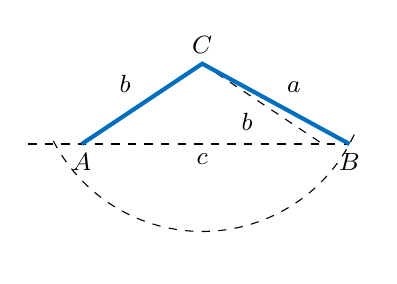
\begin{tikzpicture}[scale=0.85,every node/.style={font=\small}]
   \draw [dashed] (-0.8,0) -- (4,0);
   \draw [dashed] (1.8,1.2) -- (3.6,0) node[midway,below left] {$b$};
   \draw [dashed] ([shift={(1.8,1.2)}] -25:2.506) arc (-25:-155:2.506);
   \draw [color=sthlmBlue,line width=1.5pt] (0,0) -- (1.8,1.2) node[black,midway,above left] {$b$} --
    (4,0) node[black,midway,above right] {$a$};
   \node [below] at (1.8,0) {$c$};
   \node [below] at (0,0) {$A$};
   \node [above] at (1.8,1.2) {$C$};
   \node [below] at (4,0) {$B$};
  \end{tikzpicture}
  \end{center}

\cRed{$0\degree < A < 90\degree$, $b\;\sin\;A < a < b$ :  Two solutions}
\begin{center}
  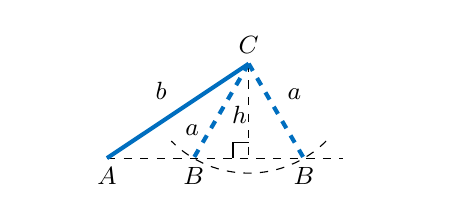
\begin{tikzpicture}[scale=1,every node/.style={font=\small}]
   \draw [white] (-1,0) -- (4,0);
   \draw [dashed] (0,0) -- (3,0);
   \draw [dashed] (1.8,1.2) -- (1.8,0);
   \node [left] at (1.9,0.55) {$h$};
   \draw (1.6,0) -- (1.6,0.2) -- (1.8,0.2);
   \draw [dashed] ([shift={(1.8,1.2)}] -45:1.39) arc (-45:-135:1.39);
   \draw [color=sthlmBlue,line width=1.5pt] (0,0) -- (1.8,1.2) node[black,midway,above left] {$b$};
   \draw [dashed,color=sthlmBlue,line width=1.5pt] (1.8,1.2) -- (2.5,0) node[black,midway,above right]
    {$a$};
   \draw [dashed,color=sthlmBlue,line width=1.5pt] (1.8,1.2) -- (1.1,0) node[black,pos=0.7,left] {$a$};
   \node [below] at (0,0) {$A$};
   \node [above] at (1.8,1.2) {$C$};
   \node [below] at (2.5,0) {$B$};
   \node [below] at (1.1,0) {$B$};
  \end{tikzpicture}
 \end{center}


\end{mysection}

\begin{mysection}{Graphs Trigonometric Functions}
  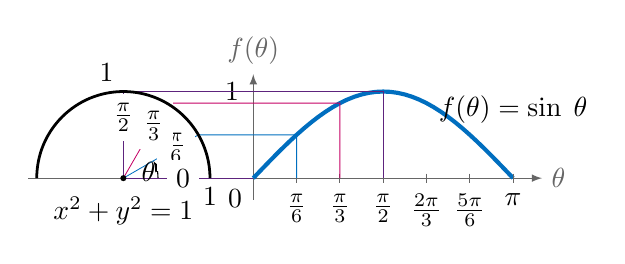
\begin{tikzpicture}[scale=0.55,5every node/.style={font=\small}]
   \begin{scope}[shift={(3,0)},color=sthlmBlue,line width=1.5pt,x=12cm/360]
	\draw[black!60,line width=0.3pt,-latex] (-5,0) -- (200,0) node[right] {$\theta$};
	\draw[black!60,line width=0.3pt,-latex] (0,-0.5) -- (0,2.4) node[above] {$f(\theta)$};
	\pgfplothandlerlineto
	\pgfplotfunction{\x}{0,5,...,180}{\pgfpointxy{\x}{2*sin(\x)}}
	\pgfusepath{stroke}
	\node[black,below left] at (0,0) {$0$};
	\foreach \pos in {30,60,90,120,150,180}
	 \draw[black!60,line width=0.3pt,shift={(\pos,0)}] (0pt,3pt) -- (0pt,-3pt);
	\foreach \pos in {2}
	 \draw[black!60,line width=0.3pt,shift={(0,\pos)}] (3pt,0pt) -- (-3pt,0pt) node[black,left]
	  {$1$};
	\node[black,below] at (30,-0.1) {$\tfrac{\pi}{6}$};
	\node[black,below] at (60,-0.1) {$\tfrac{\pi}{3}$};
	\node[black,below] at (90,-0.1) {$\tfrac{\pi}{2}$};
	\node[black,below] at (120,-0.1) {$\tfrac{2\pi}{3}$};
	\node[black,below] at (150,-0.1) {$\tfrac{5\pi}{6}$};
	\node[black,below] at (180,-0.1) {$\pi$};
	\node[black,above] at (180,1) {$f(\theta)=\sin\;\theta$};
   \end{scope}
   \draw[black!60,line width=0.3pt] (-2.2,0) -- (0,0);
   \draw[black,-latex] (0:0.8) arc (0:30:0.8);
   \draw[sthlmBlue,line width=0.3pt] (0,0) -- ++(30:2) node[black,pos=0.7,fill=white] {$\tfrac{\pi}{6}$}
	-- ++(2.268,0) -- ++(0,-1);
   \draw[sthlmRed,line width=0.3pt] (0,0) -- ++(60:2) node[black,pos=0.7,fill=white]
	{$\tfrac{\pi}{3}$} -- ++(4,0) -- ++(0,-1.732);
   \draw[sthlmPurple,line width=0.3pt] (0,0) -- ++(90:2) node[black,pos=0.7,fill=white]
	{$\tfrac{\pi}{2}$} -- ++(6,0) -- ++(0,-2);
   \draw[sthlmPurple,line width=0.3pt] (0,0) -- (3,0) node[black,pos=0.46,fill=white] {$0$};
   \draw [black,line width=1pt] (0:2) arc (0:180:2);
   \node [black,below] at (2,0) {$1$};
   \node [black,above left] at (0,2) {$1$};
   \node [black,below] at (0,-0.2) {$x^2 + y^2 = 1$};
   \node [black] at (15:0.6) {$\theta$};
   \fill (0,0) circle (2pt);
  \end{tikzpicture}

  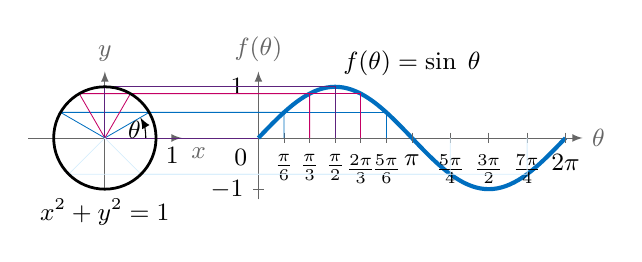
\begin{tikzpicture}[scale=0.65,every node/.style={font=\small}]
   \begin{scope}[shift={(3,0)},color=sthlmBlue,line width=1.5pt,x=6cm/360]
	\draw[black!60,line width=0.3pt,-latex] (-5,0) -- (380,0) node[right] {$\theta$};
	\draw[black!60,line width=0.3pt,-latex] (0,-1.2) -- (0,1.3) node[above] {$f(\theta)$};
	\pgfplothandlerlineto
	\pgfplotfunction{\x}{0,5,...,360}{\pgfpointxy{\x}{sin(\x)}}
	\pgfusepath{stroke}
	\node[black,below left] at (0,0) {$0$};
	\foreach \pos in {30,60,90,120,150,180,225,270,315,360}
	 \draw[black!60,line width=0.3pt,shift={(\pos,0)}] (0pt,3pt) -- (0pt,-3pt);
	\foreach \pos in {-1,1}
	 \draw[black!60,line width=0.3pt,shift={(0,\pos)}] (3pt,0pt) -- (-3pt,0pt) node[black,left]
	  {$\pos$};
	\node[black,below] at (30,-0.1) {$\tfrac{\pi}{6}$};
	\node[black,below] at (60,-0.1) {$\tfrac{\pi}{3}$};
	\node[black,below] at (90,-0.1) {$\tfrac{\pi}{2}$};
	\node[black,below] at (120,-0.1) {$\tfrac{2\pi}{3}$};
	\node[black,below] at (150,-0.1) {$\tfrac{5\pi}{6}$};
	\node[black,below] at (180,-0.1) {$\pi$};
	\node[black,below] at (225,-0.1) {$\tfrac{5\pi}{4}$};
	\node[black,below] at (270,-0.1) {$\tfrac{3\pi}{2}$};
	\node[black,below] at (315,-0.1) {$\tfrac{7\pi}{4}$};
	\node[black,below] at (360,-0.1) {$2\pi$};
	\node[black,above] at (180,1) {$f(\theta)=\sin\;\theta$};
   \end{scope}
   \draw[black!60,line width=0.3pt,-latex] (-1.5,0) -- (1.5,0) node[below right] {$x$};
   \draw[black!60,line width=0.3pt,-latex] (0,-1) -- (0,1.3) node[above] {$y$};
   \draw[black,-latex] (0:0.8) arc (0:30:0.8);
   \draw[sthlmBlue,line width=0.3pt] (0,0) -- ++(30:1);
   \draw[sthlmBlue,line width=0.3pt] (0,0) -- ++(150:1) -- ++(4.366,0) -- ++(0,-0.5);
   \draw[sthlmBlue,line width=0.3pt] (3.5,0.5) -- (5.5,0.5) -- (5.5,0);
   \draw[sthlmRed,line width=0.3pt] (0,0) -- ++(60:1);
   \draw[sthlmRed,line width=0.3pt] (0,0) -- ++(120:1) -- ++(4.5,0) -- ++(0,-0.866);
   \draw[sthlmRed,line width=0.3pt] (4,0.866) -- (5,0.866) -- (5,0);
   \draw[sthlmPurple,line width=0.3pt] (0,0) -- ++(90:1) -- ++(4.5,0) -- ++(0,-1);
   \draw[sthlmPurple,line width=0.3pt] (0,0) -- (3,0);
   \draw[sthlmLightBlue,line width=0.3pt] (0,0) -- (225:1) -- ++(7.457,0) -- ++(0,0.707);
   \draw[sthlmLightBlue,line width=0.3pt] (0,0) -- (315:1) -- ++(7.543,0) -- ++(0,0.707);
   \draw [black,line width=1pt] (0,0) circle (1);
   \node [black,below right] at (1,0) {$1$};
   \node [black,below] at (0,-1) {$x^2 + y^2 = 1$};
   \node [black] at (15:0.6) {$\theta$};
  \end{tikzpicture}
\end{mysection}

 \begin{mysection}{Sine Function}

 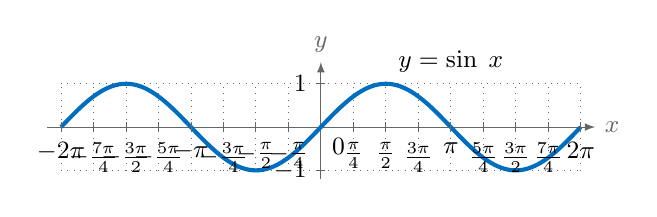
\begin{tikzpicture}[scale=0.55,every node/.style={font=\small}]
  \begin{scope}[shift={(3,0)},color=sthlmBlue,line width=1.5pt,x=6cm/360]
   \draw[black!60,line width=0.3pt,dotted] (-360,-1) grid[xstep=45,ystep=1] (360,1);
\draw[black!60,line width=0.3pt,-latex] (-380,0) -- (380,0) node[right] {$x$};
\draw[black!60,line width=0.3pt,-latex] (0,-1.2) -- (0,1.5) node[above] {$y$};
\pgfplothandlerlineto
\pgfplotfunction{\x}{-360,-355,...,360}{\pgfpointxy{\x}{sin(\x)}}
\pgfusepath{stroke}
\node[black,below right] at (0,0) {$0$};
\foreach \pos in {-360,-315,-270,-225,-180,-135,-90,-45,45,90,135,180,225,270,315,360}
 \draw[black!60,line width=0.3pt,shift={(\pos,0)}] (0pt,3pt) -- (0pt,-3pt);
\foreach \pos in {-1,1}
 \draw[black!60,line width=0.3pt,shift={(0,\pos)}] (3pt,0pt) -- (-3pt,0pt) node[black,left]
     {$\pos$};
\node[black,below] at (45,-0.1) {$\tfrac{\pi}{4}$};
\node[black,below] at (90,-0.1) {$\tfrac{\pi}{2}$};
\node[black,below] at (135,-0.1) {$\tfrac{3\pi}{4}$};
\node[black,below] at (180,-0.1) {$\pi$};
\node[black,below] at (225,-0.1) {$\tfrac{5\pi}{4}$};
\node[black,below] at (270,-0.1) {$\tfrac{3\pi}{2}$};
\node[black,below] at (315,-0.1) {$\tfrac{7\pi}{4}$};
\node[black,below] at (360,-0.1) {$2\pi$};
\node[black,below] at (-45,-0.1) {$-\tfrac{\pi}{4}$};
\node[black,below] at (-90,-0.1) {$-\tfrac{\pi}{2}$};
\node[black,below] at (-135,-0.1) {$-\tfrac{3\pi}{4}$};
\node[black,below] at (-180,-0.1) {$-\pi$};
\node[black,below] at (-225,-0.1) {$-\tfrac{5\pi}{4}$};
\node[black,below] at (-270,-0.1) {$-\tfrac{3\pi}{2}$};
\node[black,below] at (-315,-0.1) {$-\tfrac{7\pi}{4}$};
\node[black,below] at (-360,-0.1) {$-2\pi$};
\node[black,above] at (180,1) {$y=\sin\;x$};
  \end{scope}
 \end{tikzpicture}
\end{mysection}

\begin{mysection}{Cosecant Function}
  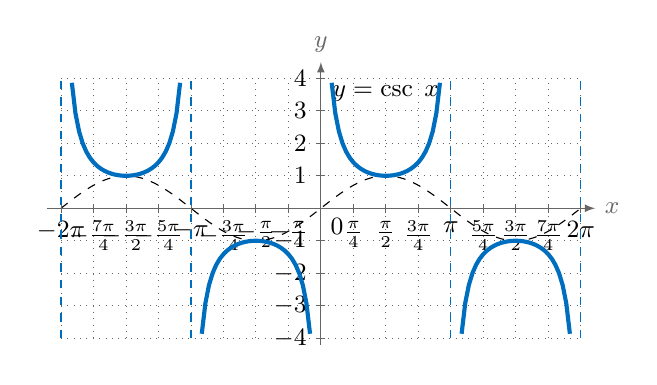
\begin{tikzpicture}[scale=0.55,every node/.style={font=\small}]
   \begin{scope}[shift={(3,0)},dashed,x=6cm/360,y=3cm/4]
    \draw[black!60,line width=0.3pt,dotted] (-360,-4) grid[xstep=45,ystep=1] (360,4);
	\draw[black!60,solid,line width=0.3pt,-latex] (-380,0) -- (380,0) node[right] {$x$};
	\draw[black!60,solid,line width=0.3pt,-latex] (0,-4.2) -- (0,4.5) node[above] {$y$};
	\pgfplothandlerlineto
	\pgfplotfunction{\x}{-360,-355,...,360}{\pgfpointxy{\x}{sin(\x)}}
	\pgfusepath{stroke}
	\node[black,below right] at (0,0) {$0$};
	\foreach \pos in {-360,-315,-270,-225,-180,-135,-90,-45,45,90,135,180,225,270,315,360}
	 \draw[black!60,solid,line width=0.3pt,shift={(\pos,0)}] (0pt,3pt) -- (0pt,-3pt);
	\foreach \pos in {-4,-3,-2,-1,1,2,3,4}
	 \draw[black!60,solid,line width=0.3pt,shift={(0,\pos)}] (3pt,0pt) -- (-3pt,0pt)
	  node[black,left] {$\pos$};
	\node[black,below] at (45,-0.1) {$\tfrac{\pi}{4}$};
	\node[black,below] at (90,-0.1) {$\tfrac{\pi}{2}$};
	\node[black,below] at (135,-0.1) {$\tfrac{3\pi}{4}$};
	\node[black,below] at (180,-0.1) {$\pi$};
	\node[black,below] at (225,-0.1) {$\tfrac{5\pi}{4}$};
	\node[black,below] at (270,-0.1) {$\tfrac{3\pi}{2}$};
	\node[black,below] at (315,-0.1) {$\tfrac{7\pi}{4}$};
	\node[black,below] at (360,-0.1) {$2\pi$};
	\node[black,below] at (-45,-0.1) {$-\tfrac{\pi}{4}$};
	\node[black,below] at (-90,-0.1) {$-\tfrac{\pi}{2}$};
	\node[black,below] at (-135,-0.1) {$-\tfrac{3\pi}{4}$};
	\node[black,below] at (-180,-0.1) {$-\pi$};
	\node[black,below] at (-225,-0.1) {$-\tfrac{5\pi}{4}$};
	\node[black,below] at (-270,-0.1) {$-\tfrac{3\pi}{2}$};
	\node[black,below] at (-315,-0.1) {$-\tfrac{7\pi}{4}$};
	\node[black,below] at (-360,-0.1) {$-2\pi$};
	\node[black,above] at (90,3) {$y=\csc\;x$};
   \end{scope}
   \begin{scope}[shift={(3,0)},color=sthlmBlue,line width=1.5pt,x=6cm/360,y=3cm/4]
	\draw[line width=0.5pt,dashed] (360,-4) -- (360,4);
	\draw[line width=0.5pt,dashed] (180,-4) -- (180,4);
	\draw[line width=0.5pt,dashed] (-360,-4) -- (-360,4);
	\draw[line width=0.5pt,dashed] (-180,-4) -- (-180,4);
	\pgfplothandlerlineto
	\pgfplotfunction{\x}{-345,-340,...,-195}{\pgfpointxy{\x}{1/sin(\x)}}
	\pgfplotfunction{\x}{-165,-160,...,-15}{\pgfpointxy{\x}{1/sin(\x)}}
	\pgfplotfunction{\x}{15,20,...,165}{\pgfpointxy{\x}{1/sin(\x)}}
	\pgfplotfunction{\x}{195,200,...,345}{\pgfpointxy{\x}{1/sin(\x)}}
	\pgfusepath{stroke}
   \end{scope}
  \end{tikzpicture}
  \end{mysection}

\begin{mysection}{Cosine Function}

  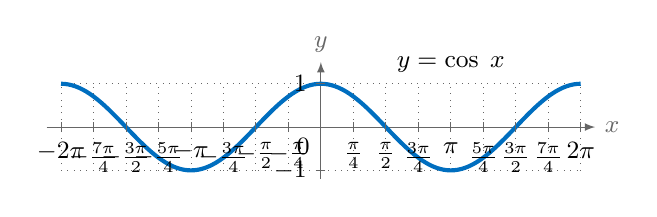
\begin{tikzpicture}[scale=0.55,every node/.style={font=\small}]
   \begin{scope}[shift={(3,0)},color=sthlmBlue,line width=1.5pt,x=6cm/360]
    \draw[black!60,line width=0.3pt,dotted] (-360,-1) grid[xstep=45,ystep=1] (360,1);
	\draw[black!60,line width=0.3pt,-latex] (-380,0) -- (380,0) node[right] {$x$};
	\draw[black!60,line width=0.3pt,-latex] (0,-1.2) -- (0,1.5) node[above] {$y$};
	\pgfplothandlerlineto
	\pgfplotfunction{\x}{-360,-355,...,360}{\pgfpointxy{\x}{cos(\x)}}
	\pgfusepath{stroke}
	\node[black,below left] at (0,0) {$0$};
	\foreach \pos in {-360,-315,-270,-225,-180,-135,-90,-45,45,90,135,180,225,270,315,360}
	 \draw[black!60,line width=0.3pt,shift={(\pos,0)}] (0pt,3pt) -- (0pt,-3pt);
	\foreach \pos in {-1,1}
	 \draw[black!60,line width=0.3pt,shift={(0,\pos)}] (3pt,0pt) -- (-3pt,0pt) node[black,left]
      {$\pos$};
	\node[black,below] at (45,-0.1) {$\tfrac{\pi}{4}$};
	\node[black,below] at (90,-0.1) {$\tfrac{\pi}{2}$};
	\node[black,below] at (135,-0.1) {$\tfrac{3\pi}{4}$};
	\node[black,below] at (180,-0.1) {$\pi$};
	\node[black,below] at (225,-0.1) {$\tfrac{5\pi}{4}$};
	\node[black,below] at (270,-0.1) {$\tfrac{3\pi}{2}$};
	\node[black,below] at (315,-0.1) {$\tfrac{7\pi}{4}$};
	\node[black,below] at (360,-0.1) {$2\pi$};
	\node[black,below] at (-45,-0.1) {$-\tfrac{\pi}{4}$};
	\node[black,below] at (-90,-0.1) {$-\tfrac{\pi}{2}$};
	\node[black,below] at (-135,-0.1) {$-\tfrac{3\pi}{4}$};
	\node[black,below] at (-180,-0.1) {$-\pi$};
	\node[black,below] at (-225,-0.1) {$-\tfrac{5\pi}{4}$};
	\node[black,below] at (-270,-0.1) {$-\tfrac{3\pi}{2}$};
	\node[black,below] at (-315,-0.1) {$-\tfrac{7\pi}{4}$};
	\node[black,below] at (-360,-0.1) {$-2\pi$};
	\node[black,above] at (180,1) {$y=\cos\;x$};
   \end{scope}
  \end{tikzpicture}
 \end{mysection}


\begin{mysection}{Secant Function}

  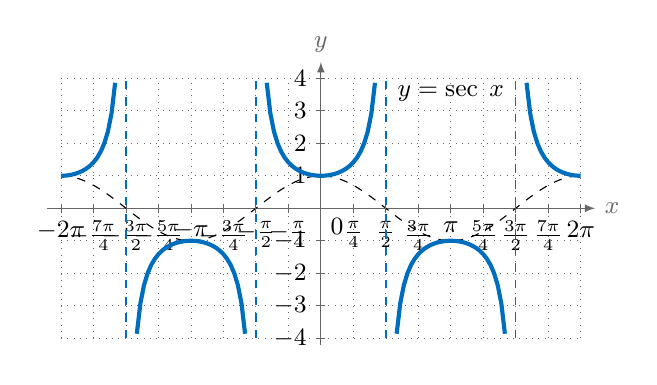
\begin{tikzpicture}[scale=0.55,every node/.style={font=\small}]
   \begin{scope}[shift={(3,0)},dashed,x=6cm/360,y=3cm/4]
    \draw[black!60,line width=0.3pt,dotted] (-360,-4) grid[xstep=45,ystep=1] (360,4);
	\draw[black!60,solid,line width=0.3pt,-latex] (-380,0) -- (380,0) node[right] {$x$};
	\draw[black!60,solid,line width=0.3pt,-latex] (0,-4.2) -- (0,4.5) node[above] {$y$};
	\pgfplothandlerlineto
	\pgfplotfunction{\x}{-360,-355,...,360}{\pgfpointxy{\x}{cos(\x)}}
	\pgfusepath{stroke}
	\node[black,below right] at (0,0) {$0$};
	\foreach \pos in {-360,-315,-270,-225,-180,-135,-90,-45,45,90,135,180,225,270,315,360}
	 \draw[black!60,solid,line width=0.3pt,shift={(\pos,0)}] (0pt,3pt) -- (0pt,-3pt);
	\foreach \pos in {-4,-3,-2,-1,1,2,3,4}
	 \draw[black!60,solid,line width=0.3pt,shift={(0,\pos)}] (3pt,0pt) -- (-3pt,0pt)
	  node[black,left] {$\pos$};
	\node[black,below] at (45,-0.1) {$\tfrac{\pi}{4}$};
	\node[black,below] at (90,-0.1) {$\tfrac{\pi}{2}$};
	\node[black,below] at (135,-0.1) {$\tfrac{3\pi}{4}$};
	\node[black,below] at (180,-0.1) {$\pi$};
	\node[black,below] at (225,-0.1) {$\tfrac{5\pi}{4}$};
	\node[black,below] at (270,-0.1) {$\tfrac{3\pi}{2}$};
	\node[black,below] at (315,-0.1) {$\tfrac{7\pi}{4}$};
	\node[black,below] at (360,-0.1) {$2\pi$};
	\node[black,below] at (-45,-0.1) {$-\tfrac{\pi}{4}$};
	\node[black,below] at (-90,-0.1) {$-\tfrac{\pi}{2}$};
	\node[black,below] at (-135,-0.1) {$-\tfrac{3\pi}{4}$};
	\node[black,below] at (-180,-0.1) {$-\pi$};
	\node[black,below] at (-225,-0.1) {$-\tfrac{5\pi}{4}$};
	\node[black,below] at (-270,-0.1) {$-\tfrac{3\pi}{2}$};
	\node[black,below] at (-315,-0.1) {$-\tfrac{7\pi}{4}$};
	\node[black,below] at (-360,-0.1) {$-2\pi$};
	\node[black,above] at (180,3) {$y=\sec\;x$};
   \end{scope}
   \begin{scope}[shift={(3,0)},color=sthlmBlue,line width=1.5pt,x=6cm/360,y=3cm/4]
	\draw[line width=0.5pt,dashed] (270,-4) -- (270,4);
	\draw[line width=0.5pt,dashed] (90,-4) -- (90,4);
	\draw[line width=0.5pt,dashed] (-270,-4) -- (-270,4);
	\draw[line width=0.5pt,dashed] (-90,-4) -- (-90,4);
	\pgfplothandlerlineto
	\pgfplotfunction{\x}{-360,-355,...,-285}{\pgfpointxy{\x}{1/cos(\x)}}
	\pgfplotfunction{\x}{-255,-250,...,-105}{\pgfpointxy{\x}{1/cos(\x)}}
	\pgfplotfunction{\x}{-75,-70,...,75}{\pgfpointxy{\x}{1/cos(\x)}}
	\pgfplotfunction{\x}{105,110,...,255}{\pgfpointxy{\x}{1/cos(\x)}}
	\pgfplotfunction{\x}{285,290,...,360}{\pgfpointxy{\x}{1/cos(\x)}}
	\pgfusepath{stroke}
   \end{scope}
  \end{tikzpicture}
\end{mysection}

\begin{mysection}{Tangent Function}
 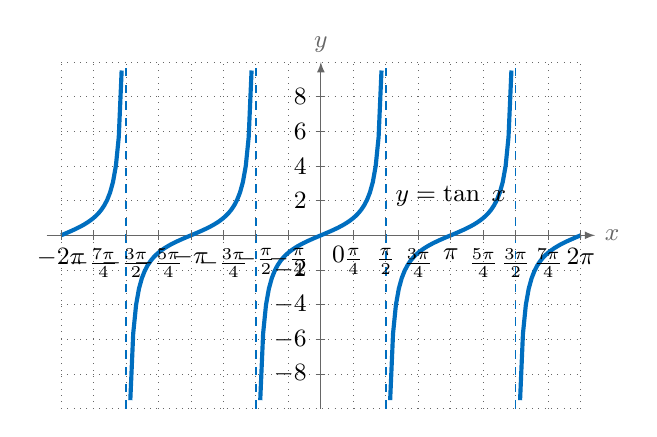
\begin{tikzpicture}[scale=0.55,every node/.style={font=\small}]
  \begin{scope}[shift={(3,0)},color=sthlmBlue,line width=1.5pt,x=6cm/360,y=4cm/10]
   \draw[black!60,line width=0.3pt,dotted] (-360,-10) grid[xstep=45,ystep=2] (360,10);
\draw[black!60,line width=0.3pt,-latex] (-380,0) -- (380,0) node[right] {$x$};
\draw[black!60,line width=0.3pt,-latex] (0,-10) -- (0,10) node[above] {$y$};
\draw[sthlmBlue,line width=0.5pt,dashed] (90,-10) -- (90,10);
\draw[sthlmBlue,line width=0.5pt,dashed] (270,-10) -- (270,10);
\draw[sthlmBlue,line width=0.5pt,dashed] (-90,-10) -- (-90,10);
\draw[sthlmBlue,line width=0.5pt,dashed] (-270,-10) -- (-270,10);
\pgfplothandlerlineto
\pgfplotfunction{\x}{-360,-356,...,-276}{\pgfpointxy{\x}{tan(\x)}}
\pgfplotfunction{\x}{-264,-260,...,-96}{\pgfpointxy{\x}{tan(\x)}}
\pgfplotfunction{\x}{-84,-80,...,84}{\pgfpointxy{\x}{tan(\x)}}
\pgfplotfunction{\x}{96,100,...,264}{\pgfpointxy{\x}{tan(\x)}}
\pgfplotfunction{\x}{276,280,...,360}{\pgfpointxy{\x}{tan(\x)}}
\pgfusepath{stroke}
\node[black,below right] at (0,0) {$0$};
\foreach \pos in {-360,-315,-270,-225,-180,-135,-90,-45,45,90,135,180,225,270,315,360}
 \draw[black!60,line width=0.3pt,shift={(\pos,0)}] (0pt,3pt) -- (0pt,-3pt);
\foreach \pos in {-8,-6,-4,-2,2,4,6,8}
 \draw[black!60,line width=0.3pt,shift={(0,\pos)}] (3pt,0pt) -- (-3pt,0pt) node[black,left]
     {$\pos$};
\node[black,below] at (45,-0.1) {$\tfrac{\pi}{4}$};
\node[black,below] at (90,-0.1) {$\tfrac{\pi}{2}$};
\node[black,below] at (135,-0.1) {$\tfrac{3\pi}{4}$};
\node[black,below] at (180,-0.1) {$\pi$};
\node[black,below] at (225,-0.1) {$\tfrac{5\pi}{4}$};
\node[black,below] at (270,-0.1) {$\tfrac{3\pi}{2}$};
\node[black,below] at (315,-0.1) {$\tfrac{7\pi}{4}$};
\node[black,below] at (360,-0.1) {$2\pi$};
\node[black,below] at (-45,-0.1) {$-\tfrac{\pi}{4}$};
\node[black,below] at (-90,-0.1) {$-\tfrac{\pi}{2}$};
\node[black,below] at (-135,-0.1) {$-\tfrac{3\pi}{4}$};
\node[black,below] at (-180,-0.1) {$-\pi$};
\node[black,below] at (-225,-0.1) {$-\tfrac{5\pi}{4}$};
\node[black,below] at (-270,-0.1) {$-\tfrac{3\pi}{2}$};
\node[black,below] at (-315,-0.1) {$-\tfrac{7\pi}{4}$};
\node[black,below] at (-360,-0.1) {$-2\pi$};
\node[black,above] at (180,1) {$y=\tan\;x$};
  \end{scope}
 \end{tikzpicture}
\end{mysection}

\begin{mysection}{Cotangent Function}
  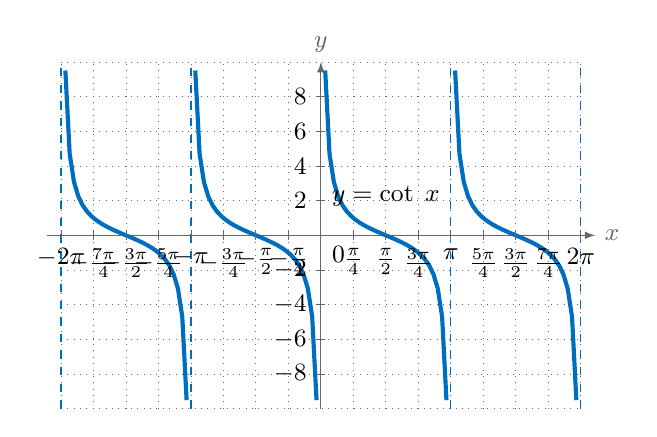
\begin{tikzpicture}[scale=0.55,every node/.style={font=\small}]
   \begin{scope}[shift={(3,0)},color=sthlmBlue,line width=1.5pt,x=6cm/360,y=4cm/10]
    \draw[black!60,line width=0.3pt,dotted] (-360,-10) grid[xstep=45,ystep=2] (360,10);
	\draw[black!60,line width=0.3pt,-latex] (-380,0) -- (380,0) node[right] {$x$};
	\draw[black!60,line width=0.3pt,-latex] (0,-10) -- (0,10) node[above] {$y$};
	\draw[sthlmBlue,line width=0.5pt,dashed] (180,-10) -- (180,10);
	\draw[sthlmBlue,line width=0.5pt,dashed] (360,-10) -- (360,10);
	\draw[sthlmBlue,line width=0.5pt,dashed] (-180,-10) -- (-180,10);
	\draw[sthlmBlue,line width=0.5pt,dashed] (-360,-10) -- (-360,10);
	\pgfplothandlerlineto
	\pgfplotfunction{\x}{-354,-348,...,-186}{\pgfpointxy{\x}{-tan(90+\x)}}
	\pgfplotfunction{\x}{-174,-168,...,-6}{\pgfpointxy{\x}{-tan(90+\x)}}
	\pgfplotfunction{\x}{6,12,...,174}{\pgfpointxy{\x}{-tan(90+\x)}}
	\pgfplotfunction{\x}{186,192,...,354}{\pgfpointxy{\x}{-tan(90+\x)}}
	\pgfusepath{stroke}
	\node[black,below right] at (0,0) {$0$};
	\foreach \pos in {-360,-315,-270,-225,-180,-135,-90,-45,45,90,135,180,225,270,315,360}
	 \draw[black!60,line width=0.3pt,shift={(\pos,0)}] (0pt,3pt) -- (0pt,-3pt);
	\foreach \pos in {-8,-6,-4,-2,2,4,6,8}
	 \draw[black!60,line width=0.3pt,shift={(0,\pos)}] (3pt,0pt) -- (-3pt,0pt) node[black,left]
      {$\pos$};
	\node[black,below] at (45,-0.1) {$\tfrac{\pi}{4}$};
	\node[black,below] at (90,-0.1) {$\tfrac{\pi}{2}$};
	\node[black,below] at (135,-0.1) {$\tfrac{3\pi}{4}$};
	\node[black,below] at (180,-0.1) {$\pi$};
	\node[black,below] at (225,-0.1) {$\tfrac{5\pi}{4}$};
	\node[black,below] at (270,-0.1) {$\tfrac{3\pi}{2}$};
	\node[black,below] at (315,-0.1) {$\tfrac{7\pi}{4}$};
	\node[black,below] at (360,-0.1) {$2\pi$};
	\node[black,below] at (-45,-0.1) {$-\tfrac{\pi}{4}$};
	\node[black,below] at (-90,-0.1) {$-\tfrac{\pi}{2}$};
	\node[black,below] at (-135,-0.1) {$-\tfrac{3\pi}{4}$};
	\node[black,below] at (-180,-0.1) {$-\pi$};
	\node[black,below] at (-225,-0.1) {$-\tfrac{5\pi}{4}$};
	\node[black,below] at (-270,-0.1) {$-\tfrac{3\pi}{2}$};
	\node[black,below] at (-315,-0.1) {$-\tfrac{7\pi}{4}$};
	\node[black,below] at (-360,-0.1) {$-2\pi$};
	\node[black,above] at (90,1) {$y=\cot\;x$};
   \end{scope}
  \end{tikzpicture}
  \end{mysection}

\begin{mysection}{Algebraic Limit Theorems}

\begin{tabular}{@{}ll@{}}
\cRed{ALTC} & \texttt{Algebraic Limit Theorem of a Constant} \\
& \qquad $\displaystyle \lim_{x \to c} \left[ A \right] = A$\\
& \\
\cRed{ALTS} & \texttt{Algebraic Limit Theorem of a Sum} \\
& \qquad $\displaystyle \lim_{x \to c} \left[ g(x)+h(x) \right] = \displaystyle \lim_{x \to c} g(x)+ \displaystyle \lim_{x \to c} h(x)$\\
& \\
\cRed{ALTD} & \texttt{Algebraic Limit Theorem of a Difference} \\
& \qquad $\displaystyle \lim_{x \to c} \left[ g(x)-h(x) \right] = \displaystyle \lim_{x \to c} g(x)- \displaystyle \lim_{x \to c} h(x)$\\
& \\
\cRed{ALTPr} & \texttt{Algebraic Limit Theorem of a Product} \\
& \qquad $\displaystyle \lim_{x \to c} \left[ g(x) \cdot h(x) \right] = \displaystyle \lim_{x \to c} g(x) \cdot \displaystyle \lim_{x \to c} h(x)$\\
& \\
\cRed{ALTQ} & \texttt{Algebraic Limit Theorem of a Quotient} \\
& \qquad $\displaystyle \lim_{x \to c} \left[ \dfrac{g(x)}{h(x)}\right] =  \dfrac{\displaystyle \lim_{x \to c} g(x)}{\displaystyle \lim_{x \to c} h(x)}$\\
& \\
\end{tabular}

\end{mysection}

\begin{mysection}{Differentiation by First Principles}

\begin{tabular}{@{}ll@{}}
\cRed{DFP}			& \texttt{Differentiation by first principles} \\
						& \qquad $f'(x) = \displaystyle \lim_{\Delta x \to 0} \dfrac{f(x+\Delta x) - f(x)}{\Delta x}$\\
						&
\end{tabular}
\end{mysection}

\begin{mysection}{Notations}

\begin{tabular}{@{}ll@{}}
& \texttt{Leibniz's first derivative} \\
& \qquad $\dfrac{\dy}{\dx} = \dfrac{d \left[f(x) \right]}{\dx}= \dfrac{d}{\dx} \left[f(x) \right]$\\
& \\
& \texttt{Leibniz's second derivative} \\
& \qquad $\dfrac{\dd^{2}y}{\dx^{2}}$\\
& \\
& \texttt{Leibniz's nth derivative} \\
& \qquad $\dfrac{\dd^{n}y}{\dx^{n}}$\\
& \\
& \texttt{Leibniz's evaluate derivative at $x=a$} \\
& \qquad $\dydx\left.{\!\!\frac{}{}}\right|_{x=a} = \dydx(a)$\\
& \\
& \texttt{LaGrange's first derivative} \\
& \qquad $f'(x)$\\
& \\
& \texttt{LaGrange's second derivative} \\
& \qquad $f''(x)$\\
& \\
& \texttt{LaGrange's nth derivative} \\
& \qquad $f^{(n)}(x)$\\
& \\
& \texttt{LaGrange's evaluate derivative at $x=a$} \\
& \qquad $f'(a)$\\
& \\
& \texttt{Euler's first derivative} \\
& \qquad $Df =D_{x}f $\\
& \\
& \texttt{Euler's second derivative} \\
& \qquad $D^{2}f=D_{x}^{2}f$\\
& \\
& \texttt{Euler's nth derivative} \\
& \qquad $D^{n}f= D_{x}^{n}$\\
& \\
\end{tabular}

\end{mysection}

\begin{mysection}{Differentiation Structural Rules}
\begin{tabular}{@{}ll@{}}
\cRed{DS}			& \texttt{Derivative of a sum} \\
						& $[f(x) + g(x)]'= f'(x) + g'(x) $\\
						& \\
						& $\dfrac{\dd}{\dx} \left[f(x) + g(x) \right]= \dfrac{\dd}{\dx} \left[f(x) \right] + \dfrac{\dd}{\dx} \left[g(x) \right] $\\
						& \\
\cRed{DD}			& \texttt{Derivative of a difference} \\
						& $\left[f(x) - g(x) \right]'= f'(x) - g'(x) $\\
						& \\
						& $\dfrac{\dd}{\dx} \left[f(x) - g(x) \right]= \dfrac{\dd}{\dx} \left[f(x) \right] - \dfrac{\dd}{\dx} \left[g(x) \right] $\\
						& \\
\cRed{DPr}			& \texttt{Derivative of a product "Product Rule"} \\
						& $\left[f(x)g(x) \right]' = f'(x)g(x) + f(x)g'(x) $\\
						& \\
						& $\dfrac{\dd}{\dx} \left[f(x)g(x) \right]= \dfrac{\dd}{\dx} \left[f(x) \right]g(x) + f(x)\dfrac{\dd}{\dx} \left[g(x)\right] $\\
						& \\
\cRed{DQ}			& \texttt{Derivative of a quotient "Quotient Rule"} \\
						& $\left[ \dfrac{f(x)}{g(x)} \right]'= \dfrac{f'(x)g(x)-f(x)g'(x)}{\left[g(x)\right]^2}$\\
						& \\
						& $\dfrac{\dd}{\dx} \left[ \dfrac{f(x)}{g(x)} \right]= \dfrac{\dfrac{\dd}{\dx}\left[f(x)\right]g(x)-f(x) \dfrac{\dd}{\dx} \left[g(x)\right] }{\left[g(x)\right]^2}$\\
						& \\
\cRed{DCF}			& \texttt{Derivative of a composite function}\\
						& $ \left[f \left( g(x) \right) \right]'= \left[g(x) \right]' \left[f\left(g(x)\right)\right]'$\\
						& \\
						& $\dfrac{\dd}{\dx} \left[f \left( g(x) \right) \right]= \dfrac{\dd}{\dx} \left[g(x) \right] \dfrac{\dd}{\dx} \left[f\left(g(x)\right)\right]$\\
						&
\end{tabular}
\end{mysection}

\begin{mysection}{Differentiation Monomial Rules}

\begin{tabular}{@{}ll@{}}
\cRed{DC}			& \texttt{Derivative of a constant} \\
						& $\left[c \right]' = 0$ \\
						& \\
						& $\dfrac{\dd}{\dx} \left[c \right]=0$\\
						& \\
\cRed{DCM}			& \texttt{Derivative of a constant multiple} \\
						& $\left[c f(x) \right]'= c \left[f(x)\right]'$\\
						& \\
						& $\dfrac{\dd}{\dx}\left[c f(x) \right]= c \dfrac{\dd}{\dx}\left[f(x)\right]$\\
						& \\
\cRed{DPo}			& \texttt{Derivative of a power "Power Rule"} \\
						& $\left[x^n \right]'= n x^{n-1}$\\
						& \\
						& $\dfrac{\dd}{\dx} \left[x^n \right]= n x^{n-1}$\\
						&
\end{tabular}

\end{mysection}

\begin{mysection}{Differentiation Exponential and Logarithmic Function Rules}

\begin{tabular}{@{}ll@{}}
\cRed{DExp}		& \texttt{Derivative of an exponential function} \\
						& $\dfrac{\dd}{\dx}\left[ a^x \right] =a^{x} \ln a$\\
						& \\
\cRed{DNExp}		& \texttt{Derivative of a natural} \\
						& \texttt{exponential function} \\
						& $\dfrac{\dd}{\dx} \left[e^x \right]=e^{x}$\\
						& \\
\cRed{DL}			& \texttt{Derivative of a logarithmic function} \\
						& $\dfrac{\dd}{\dx} \left[ \log_{a}x \right]= \frac{1}{x \ln a}$\\
						& \\
\cRed{DNL}			& \texttt{Derivative of a natural}\\
						& \texttt{logarithmic function} \\
						& $\dfrac{\dd}{\dx} \left[\ln x \right]= \frac{1}{x}$\\
						&

\end{tabular}
\end{mysection}

\begin{mysection}{Differentiation Trigonometric Function Rules}

\begin{tabular}{@{}ll@{}}
\cRed{DSin}		& \texttt{Derivative of a sine function} \\
						& $\dfrac{\dd}{\dx}(\sin x)= \cos x$\\
						& \\
\cRed{DCos}		& \texttt{Derivative of a cosine function} \\
						& $\dfrac{\dd}{\dx}(\cos x)= - \sin x$\\
						& \\
\cRed{DTan}		& \texttt{Derivative of a tangent function} \\
						& $\dfrac{\dd}{\dx} (\tan x)= \sec^2 x$\\
						& \\
\cRed{DCsc}		& \texttt{Derivative of a cosecant function} \\
						& $\dfrac{\dd}{\dx}(\csc x)= - \csc x \cot x$\\
						& \\
\cRed{DSec}		& \texttt{Derivative of a secant function} \\
						& $\dfrac{\dd}{\dx} (\sec x)= \sec x \tan x$\\
						& \\
\cRed{DCot}		& \texttt{Derivative of a cotangent function} \\
						& $\dfrac{\dd}{\dx} (\cot x)= -\csc^2 x$\\
						&
\end{tabular}
\end{mysection}

\vfill
\rule{0.3\linewidth}{0.25pt}
\scriptsize


v42.org https://plus.google.com/+MarkHendryOlsonV42\\
Trig images: http://bit.ly/mecmath-trigbook\\
Pascal's triangle: http://bit.ly/1kIYJ9H \\


\end{multicols}
\end{document}
